% Created 2022-09-14 Wed 15:26
% Intended LaTeX compiler: xelatex
\documentclass[table,10pt,aspectratio=169]{beamer}

\RequirePackage{etex}
\RequirePackage[l2tabu,orthodox]{nag}            %% Warn about obsolete commands and packages
\RequirePackage{amsmath,amsfonts,amssymb,amsthm} %% Math
\RequirePackage{ifxetex,ifluatex}                %% Detect XeTeX and LuaTeX
\RequirePackage{fixltx2e}                        %% provides \textsubscript
\RequirePackage{xspace}
\RequirePackage{graphicx}
\RequirePackage{comment}
\RequirePackage{url}
\RequirePackage{relsize}
\RequirePackage{booktabs}
\RequirePackage{tabularx}
\RequirePackage[normalem]{ulem}
\RequirePackage[all]{xy}
\RequirePackage{etoolbox}

%%%
%%% Code Listings
%%%

\RequirePackage{listings}
\lstdefinelanguage{Sage}[]{Python}{morekeywords={True,False,sage,cdef,cpdef,ctypedef,self},sensitive=true}

\lstset{frame=none,
  showtabs=False,
  showspaces=False,
  showstringspaces=False,
  commentstyle={\color{gray}},
  keywordstyle={\color{mLightBrown}\textbf},
  stringstyle ={\color{mDarkBrown}},
  frame=single,
  basicstyle=\tt\scriptsize\relax,
  backgroundcolor=\color{gray!190!black},
  inputencoding=utf8,
  literate={…}{{\ldots}}1,
  belowskip=0.0em,
}

\makeatletter
\patchcmd{\@verbatim}
  {\verbatim@font}
  {\verbatim@font\scriptsize}
  {}{}
\makeatother


%%%
%%% Pseudocode
%%%

\let\nl\undefine
\let\procedure\relax
\let\endprocedure\relax
\usepackage{algorithm2e}

%%%
%%% Tikz
%%%

\RequirePackage{tikz,pgfplots}
\pgfplotsset{compat=newest}

\usetikzlibrary{calc}
\usetikzlibrary{arrows}
\usetikzlibrary{automata}
\usetikzlibrary{positioning}
\usetikzlibrary{decorations.pathmorphing}
\usetikzlibrary{backgrounds}
\usetikzlibrary{fit,}
\usetikzlibrary{shapes.symbols}
\usetikzlibrary{chains}
\usetikzlibrary{shapes.geometric}
\usetikzlibrary{shapes.arrows}
\usetikzlibrary{graphs}

%% Cache but disable by default

\usetikzlibrary{external}
\tikzset{external/export=false}

\definecolor{DarkPurple}{HTML}{332288}
\definecolor{DarkBlue}{HTML}{6699CC}
\definecolor{LightBlue}{HTML}{88CCEE}
\definecolor{DarkGreen}{HTML}{117733}
\definecolor{DarkRed}{HTML}{661100}
\definecolor{LightRed}{HTML}{CC6677}
\definecolor{LightPink}{HTML}{AA4466}
\definecolor{DarkPink}{HTML}{882255}
\definecolor{LightPurple}{HTML}{AA4499}
\definecolor{DarkBrown}{HTML}{604c38}
\definecolor{DarkTeal}{HTML}{23373b}
\definecolor{LightBrown}{HTML}{EB811B}
\definecolor{LightGreen}{HTML}{14B03D}
\definecolor{DarkOrange}{HTML}{FFDD00}

\pgfplotsset{width=1.0\textwidth,
  height=0.6\textwidth,
  cycle list={%
    solid,LightGreen,thick\\%
    dotted,LightRed,very thick\\%
    dashed,DarkBlue,thick\\%
    dashdotted,DarkPink,thick\\%
    dashdotdotted,LightGreen,thick\\%
    loosely dotted,very thick\\%
    loosely dashed,DarkBlue,very thick\\%
    loosely dashdotted,DarkPink,very thick\\%
    \\%
    DarkBrown,thick\\%
  },
  legend pos=north west,
  legend cell align={left}}

\pgfplotsset{select coords between index/.style 2 args={
    x filter/.code={
        \ifnum\coordindex<#1\def\pgfmathresult{}\fi
        \ifnum\coordindex>#2\def\pgfmathresult{}\fi
    }
}}

%%%
%%% SVG (Inkscape)
%%%

\ifxetex % chktex 1
\providecommand{\executeiffilenewer}[3]{%
  {\immediate\write18{#3}} % hack
}
\else
\providecommand{\executeiffilenewer}[3]{%
  \ifnum\pdfstrcmp{\pdffilemoddate{#1}}%
    {\pdffilemoddate{#2}}>0%
    {\immediate\write18{#3}}
  \fi%
}
\fi

\providecommand{\includesvg}[2][1.0\textwidth]{%
 \executeiffilenewer{#1.svg}{#1.pdf}%
 {inkscape -z -D --file=#2.svg --export-pdf=#2.pdf --export-latex --export-area-page}%
 \def\svgwidth{#1} 
 \input{#2.pdf_tex}%
} 

%%%
%%% Metropolis Theme
%%%

\usetheme{metropolis}
\metroset{color/block=fill}
\metroset{numbering=none}
\metroset{outer/progressbar=foot}
\metroset{titleformat=smallcaps}

\setbeamercolor{description item}{fg=mLightBrown}
% \setbeamerfont{alerted text}{series=\bfseries}
\setbeamerfont{footnote}{size=\scriptsize}
\setbeamercolor{example text}{fg=mDarkBrown}
\setbeamercolor{block title alerted}{fg=white, bg=mDarkBrown}
\setbeamertemplate{bibliography item}[text]

\renewcommand*{\UrlFont}{\ttfamily\relax}

%%%
%%% UTF-8 & Fonts
%%% 

\RequirePackage{unicodesymbols} % after metropolis which loads fontspec

\setmonofont[BoldFont={Cousine Bold},
             ItalicFont={Cousine Italic},
             BoldItalicFont={Cousine Bold Italic},
             Scale=0.9]{Cousine}             
%%%
%%% BibLaTeX
%%%

\RequirePackage[backend=bibtex,
            style=alphabetic,
            maxnames=8,maxbibnames=8,maxalphanames=8,
            citestyle=alphabetic]{biblatex}

\bibliography{local.bib,abbrev3.bib,crypto_crossref.bib,rfc.bib,jacm.bib,dcc.bib}

\DeclareFieldFormat{title}{\alert{#1}}
\DeclareFieldFormat[book]{title}{\alert{#1}}
\DeclareFieldFormat[thesis]{title}{\alert{#1}}
\DeclareFieldFormat[inproceedings]{title}{\alert{#1}}
\DeclareFieldFormat[incollection]{title}{\alert{#1}}
\DeclareFieldFormat[article]{title}{\alert{#1}}
\DeclareFieldFormat[misc]{title}{\alert{#1}}

%%% 
%%% Microtype
%%%

\IfFileExists{upquote.sty}{\RequirePackage{upquote}}{}
\IfFileExists{microtype.sty}{\RequirePackage{microtype}}{}

\setlength{\parindent}{0pt}                   %%
\setlength{\parskip}{6pt plus 2pt minus 1pt}  %%
\setlength{\emergencystretch}{3em}            %% prevent overfull lines
\setcounter{secnumdepth}{0}                   %%

%%%
%%% Maths
%%%

\DeclareMathOperator{\Vol}{Vol}
\DeclareMathOperator{\GH}{GH}
\renewcommand{\vec}[1]{\ensuremath{\mathbf{#1}}\xspace}
\newcommand{\norm}[1]{\left\lVert#1\right\rVert}
\providecommand{\mat}[1]{\ensuremath{\vec{#1}}\xspace}
\providecommand{\ring}[0]{\ensuremath{\mathcal{R}}\xspace}

%%% Local Variables:
%%% mode: latex
%%% End:
\usepackage{graphicx}
\usepackage{longtable}
\usepackage{wrapfig}
\usepackage{rotating}
\usepackage[normalem]{ulem}
\usepackage{amsmath}
\usepackage{amssymb}
\usepackage{capt-of}
\usepackage{hyperref}
\usepackage{booktabs}
\usepackage{microtype}
\usepackage{newunicodechar}
\usepackage[notions,operators,sets,keys,ff,adversary,primitives,complexity,asymptotics,lambda,landau,advantage]{cryptocode}
\usepackage[capitalize]{cleveref}
\usepackage[english]{babel}
\usepackage{xspace}
\usepackage{units}
\usepackage{nicefrac}
\usepackage{gensymb}
\usepackage{amsthm}
\usepackage{amsmath}
\usepackage{amssymb}
\usepackage{xcolor}
\usepackage{listings}
\usepackage[color=cyan!0!magenta!4!yellow!16]{todonotes}
\tikzset{external/optimize=false}
\tikzexternalize[prefix=cache/]
\def\robl{\rowcolor{DarkBlue!20}}
\def\rore{\rowcolor{DarkRed!20}}
\def\rogr{\rowcolor{gray!20}}
\def\enumworstfit{\(1/(2e)\, \beta \log(\beta) - \beta + 16.1\)}
\def\enumavgfit{\(1/8\,\beta \log(\beta) - 0.75\beta + 2.3\)}
\def\qenumworstfit{\(1/(4e)\, \beta \log(\beta) - 0.5\beta + 8\)}
\institute{2022: Royal Holloway, University of London, 2023: King's College London \& SandboxAQ}
\usetheme{default}
\author{Martin R. Albrecht}
\date{}
\title{Estimating the Difficulty of Breaking Lattice-Based Cryptography}
\subtitle{with a focus on LWE}
\hypersetup{
pdfauthor={Martin R. Albrecht},
pdftitle={Estimating the Difficulty of Breaking Lattice-Based Cryptography},
pdfkeywords={},
pdfsubject={},
pdfcreator={Emacs 28.1.91 (Org mode 9.5.4)},
pdflang={English},
colorlinks,
citecolor=gray,
filecolor=gray,
linkcolor=gray,
urlcolor=gray
}
\begin{document}

\maketitle

\begin{frame}[label={sec:org1ee5670}]{The Plan}
\begin{itemize}
\item Introduce estimating the cost of solving LWE-based schemes
\begin{itemize}
\item strategies (primal and dual lattice attacks)
\item lattice reduction
\item finding short vectors
\item quantum considerations
\end{itemize}
\item Introduce usage of "lattice estimator" along the way
\begin{itemize}
\item highlight limitations\footnote{Most of what I know about running open-source projects, I learned from William Stein who responded with "Easy, implement it and send us a patch!" when asked "How do I do … in SageMath?"}
\end{itemize}
\end{itemize}

\begin{alertblock}{}
\begin{center}
\url{https://github.com/malb/lattice-estimator/}
\end{center}
\end{alertblock}
\end{frame}

\begin{frame}[label={sec:org235cd0f},fragile]{Example}
 \lstset{language=Python,label= ,caption= ,captionpos=b,numbers=none}
\begin{lstlisting}
_ = LWE.estimate.rough(Kyber768)
\end{lstlisting}

\begin{verbatim}
usvp                 :: rop: ≈2^182.2, red: ≈2^182.2, δ: 1.002902, β: 624, d: 1427, tag: usvp
dual_hybrid          :: rop: ≈2^184.3, mem: ≈2^180.8, m: 705, β: 630, d: 1451, ↻: 1, ζ: 22, tag: dual_hybrid
\end{verbatim}


\lstset{language=Python,label= ,caption= ,captionpos=b,numbers=none}
\begin{lstlisting}
_ = LWE.estimate(Kyber768)
\end{lstlisting}

\begin{verbatim}
arora-gb             :: rop: ≈2^inf, dreg: 94, mem: ≈2^513.9, t: 2, m: ≈2^inf, …
bkw                  :: rop: ≈2^238.3, m: ≈2^225.5, mem: ≈2^226.5, b: 19, t1: 1, t2: 17, ℓ: 18, …
usvp                 :: rop: ≈2^204.9, red: ≈2^204.9, δ: 1.002902, β: 624, d: 1427, tag: usvp
bdd                  :: rop: ≈2^201.0, red: ≈2^200.0, svp: ≈2^200.0, β: 606, η: 641, d: 1425, tag: bdd
bdd_hybrid           :: rop: ≈2^201.0, red: ≈2^200.0, svp: ≈2^200.0, β: 606, η: 641, …
bdd_mitm_hybrid      :: rop: ≈2^356.7, red: ≈2^355.8, svp: ≈2^355.6, β: 623, η: 2, ζ: 189, …
dual                 :: rop: ≈2^214.2, mem: ≈2^133.4, m: 723, β: 653, d: 1491, ↻: 1, tag: dual
dual_hybrid          :: rop: ≈2^206.4, mem: ≈2^201.9, m: 701, β: 625, d: 1437, ↻: 1, ζ: 32, tag: dual_hybrid
\end{verbatim}
\end{frame}

\section{Computational Problems}
\label{sec:org4121d54}
\begin{frame}[label={sec:org2c99efa}]{Learning with Errors}
Given \((\mathbf{A},\vec{c})\), find \(\vec{s}\) when

\[
\left(\begin{array}{c}
\\
\\
\\ 
\vec{c} \\
\\
\\
\\
\end{array} \right) \equiv \left(
\begin{array}{ccc}
\leftarrow & n & \rightarrow \\
\\
\\ 
& \mathbf{A} & \\
\\
\\
\\
\end{array} \right) \cdot \left( \begin{array}{c}
\\\
\\
\vec{s} \\
\\
\\
\end{array} \right) + \left(
\begin{array}{c}
\\
\\
\\ 
\vec{e} \\
\\
\\
\\
\end{array} 
\right) \bmod q
\]

for \(\vec{c} \in \ZZ_q^{m}\), \(\mat{A} \in \ZZ_q^{m \times n}\), and \(\vec{s} \in \ZZ^{n}\) and \(\vec{e} \in \ZZ^{m}\) having small entries.
\end{frame}

\begin{frame}[label={sec:orga91b2af}]{Learning with Errors}
Given \((\mathbf{A},\vec{c})\), find \(\vec{s}\) when

\[
\left(\begin{array}{c}
\\
\\
\\ 
\vec{c} \\
\\
\\
\\
\end{array} \right) \equiv \left(
\begin{array}{ccc}
\leftarrow & n & \rightarrow \\
\\
\\ 
& \mathbf{A} & \\
\\
\\
\\
\end{array} \right) \cdot \left( \begin{array}{c}
\\\
\\
\vec{s} \\
\\
\\
\end{array} \right) + \left(
\begin{array}{c}
\\
\\
\\ 
\vec{e} \\
\\
\\
\\
\end{array} 
\right) \bmod q
\]

for \(\vec{c} \in \ZZ_q^{m}\), \(\mat{A} \in \ZZ_q^{m \times n}\), and \(\vec{s} \in \ZZ^{n}\) and \(\vec{e} \in \ZZ^{m}\) \alert{having small entries}.
\end{frame}

\begin{frame}[label={sec:org719bcd7},fragile]{"Having Small Entries"}
 \begin{columns}
\begin{column}{0.5\columnwidth}
\begin{description}
\item[{Discrete Gaussian}] the classic, annoying to sample from; ➡
\item[{Binomial}] \(\sum_{0 \leq i < \eta} (b_{i} - b_{\eta+i}) \mid b_{j} \sample \bin\)
\item[{Small Uniform}] \(\sample [a,\ldots,b] \mid a,b \in \NN\)
\end{description}
\end{column}

\begin{column}{0.5\columnwidth}
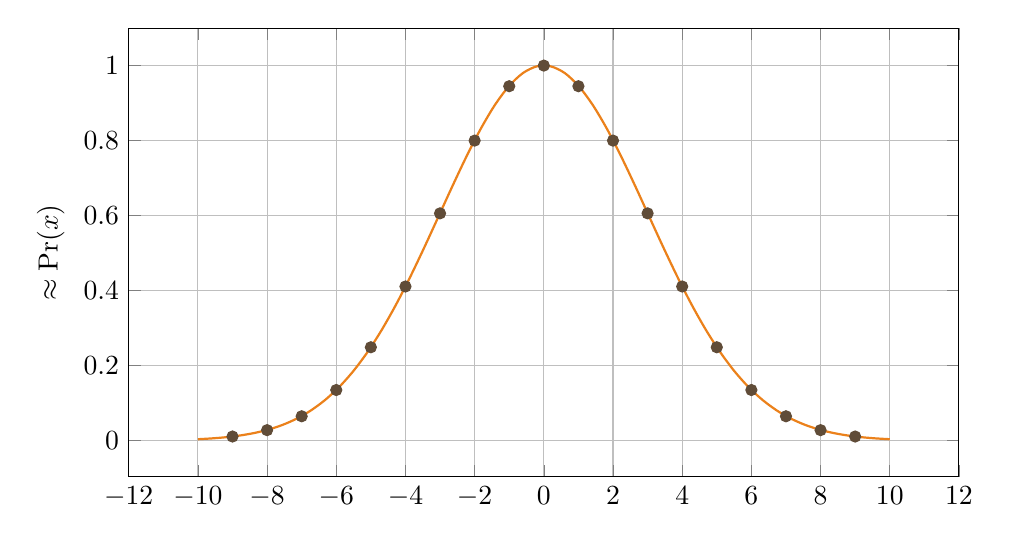
\begin{tikzpicture}
  \begin{axis}[
    domain=-10:10,
    grid=major,smooth,
    % xlabel=$x$,
    ylabel=$\approx \textnormal{Pr}(x)$,
    ]
    \addplot[color=LightBrown,thick,samples=50,smooth]{exp(-(x^2)/18)};
    \addplot[color=DarkBrown,only marks] coordinates {
      (-9, 0.011)
      (-8, 0.028)
      (-7, 0.065)
      (-6, 0.135)
      (-5, 0.249)
      (-4, 0.411)
      (-3, 0.606)
      (-2, 0.800)
      (-1, 0.945)
      (0, 1.000)
      (1, 0.945)
      (2, 0.800)
      (3, 0.606)
      (4, 0.411)
      (5, 0.249)
      (6, 0.135)
      (7, 0.065)
      (8, 0.028)
      (9, 0.011)
    };
  \end{axis}
\end{tikzpicture}
\end{column}
\end{columns}

\lstset{language=Python,label= ,caption= ,captionpos=b,numbers=none}
\begin{lstlisting}
from estimator import *
ND.DiscreteGaussian(stddev=2), ND.CenteredBinomial(eta=8), ND.Uniform(-3, 3)
\end{lstlisting}

\begin{verbatim}
(D(σ=2.00), D(σ=2.00), D(σ=2.00))
\end{verbatim}


\begin{itemize}
\item Literature assumes these all behave essentially the same under attacks
\item No loss in security if secret \(\vec{s}\) and error \(\vec{e}\) have same distribution \cite{C:ACPS09}
\end{itemize}
\end{frame}

\begin{frame}[label={sec:org3d147cd},fragile]{Estimator}
 \lstset{language=Python,label= ,caption= ,captionpos=b,numbers=none}
\begin{lstlisting}
Kyber768 = LWEParameters(
    n=3 * 256,
    q=3329,
    Xs=ND.CenteredBinomial(2),
    Xe=ND.CenteredBinomial(2),
    m=3 * 256,
    tag="Kyber 768",
)
\end{lstlisting}

\begin{alertblock}{Q: "How do I do NTRU?"}
A: "Easy, implement it and send us a patch."

We do not offer \texttt{NTRUParameters}, but you can hack it in using \texttt{LWEParameters}
\end{alertblock}
\end{frame}

\section{Approaches}
\label{sec:orgae3b24b}
\begin{frame}[label={sec:orgf0c8d9f}]{Unique SVP/BDD: Translation}
We can reformulate \(\vec{c} - \mathbf{A} \cdot \vec{s} \equiv \vec{e} \bmod q\)  over the Integers as:
\[
  \begin{pmatrix}
    q\mathbf{I} & -\mathbf{A}\\
    0 & \mathbf{I}\\
  \end{pmatrix} \cdot
  \begin{pmatrix}
    \mathbf{*}\\
    \mathbf{s}
  \end{pmatrix} +
  \begin{pmatrix}
    \vec{c}\\
    \vec{0}
  \end{pmatrix} = 
  \begin{pmatrix}
    \vec{e}\\
    \vec{s}
  \end{pmatrix}
\]
Alternatively:
\[
  \mathbf{B} = \begin{pmatrix}
    q\mathbf{I} & -\mathbf{A} & \vec{c}\\
    0 & \mathbf{I} & 0\\
    0 & 0 & 1\\
  \end{pmatrix}, \qquad
  \mathbf{B} \cdot
  \begin{pmatrix}
    \vec{*}\\
    \vec{s}\\
    1
  \end{pmatrix} = 
  \begin{pmatrix}
    \vec{e}\\
    \vec{s}\\
    1
  \end{pmatrix}
\]

In other words, there exists an integer-linear combination of the columns of \(\mathbf{B}\) that produces a vector with “unusually” small entries \(\rightarrow\) a unique shortest vector.
\end{frame}

\begin{frame}[label={sec:org3211c7c}]{Unique SVP: Computational Problem}
\begin{block}{Unique Shortest Vector Problem for \(q\)-ary Lattices}
Find a unique shortest vector amongst the integer combinations of the columns of:
\[
  \mat{B} = \begin{pmatrix}
 q\mat{I} & -\mat{A} & \vec{c}\\
 0        & \mat{I}  & 0\\
 0        & 0        & 1\\
  \end{pmatrix}
\]
where \(\mat{B} \in \ZZ^{d \times d}\).
\end{block}

\begin{block}{Decision Variant}
Decide if \(\mat{B}\) has an unusually short vector.
\end{block}
\end{frame}

\begin{frame}[label={sec:orgfbdab3c}]{Approx SVP/SIS: Translation}
\begin{itemize}
\item Consider \(\vec{c} \equiv \mat{A} \cdot \vec{s} + \vec{e} \bmod q\) with both \(\vec{s}\) and \(\vec{e}\) short or \(\vec{c}\) uniform.
\item Let \(\vec{u}_{i}\) be short vectors such that \(\vec{v}_i^{T} \coloneqq \vec{u}_i^{T} \cdot \mat{A} \bmod q\)  is also short.
\item Compare:
\begin{itemize}
\item \(\vec{u}_i^{T} \cdot \vec{c} \equiv \vec{u}_i^{T} \cdot \vec{A} \cdot \vec{s} + \vec{u}_i^{T} \cdot \vec{e} \equiv \vec{v}_i^{T} \cdot \vec{s} + \vec{u}_i^{T}\cdot \vec{e}\)  which is somewhat short
\item \(\vec{u}_i^{T} \cdot \vec{c}\) which is uniform
\end{itemize}
\item The shorter \((\vec{u}_i,\vec{v}_{i})\) the fewer samples of \(\vec{u}_i^{T} \cdot \vec{c}\) we need to consider
\item Note
\end{itemize}
\[
  \begin{pmatrix}
    q\mathbf{I} & \mathbf{A}^{T}\\
    0 & \mathbf{I}\\
  \end{pmatrix} \cdot
  \begin{pmatrix}
    \vec{*}\\
    \vec{u}_{i}
  \end{pmatrix} = 
  \begin{pmatrix}
    \vec{v}_{i}\\
    \vec{u}_{i}
  \end{pmatrix}  
\]
\end{frame}

\begin{frame}[label={sec:org70a5cf0}]{Approx SVP: Computational Problem}
\begin{block}{Short Vectors Problem for \(q\)-ary Lattices}
Find vectors \((\vec{u}_i, \vec{v}_i)\) of norm \(\|(\vec{u}_i, \vec{v}_i)\| \leq \beta\) amongst the integer combinations of the columns of:
\[
  \mat{B} = \begin{pmatrix}
 q\mat{I} & \mat{A}^{T}\\
 0        & \mat{I}\\
  \end{pmatrix}
\]
where \(\mat{B} \in \ZZ^{d \times d}\).
\end{block}

\begin{block}{Search Variant}
Can extend this distinguishing attack to recover \(\vec{s}\): guess a component and run the distinguisher
\end{block}
\end{frame}

\begin{frame}[label={sec:org6d12475}]{Lattice Reduction <3 Combinatorics: Hybrid Attacks}
Both approaches can be augmented with a combinatorial step
\begin{itemize}
\item guess parts of the secret and run the lattice attack on a smaller dimensional lattice
\item due to linearity costs are additive not multiplicative, i.e.\[\approx T_{guess} + T_{lattice}\]
\end{itemize}
\end{frame}

\begin{frame}[label={sec:orgc4824e5},fragile]{Estimator (Primal)}
 \textbf{plain uSVP}

\lstset{language=Python,label= ,caption= ,captionpos=b,numbers=none}
\begin{lstlisting}
LWE.primal_usvp(Kyber768)
\end{lstlisting}

\begin{verbatim}
rop: ≈2^204.9, red: ≈2^204.9, δ: 1.002902, β: 624, d: 1427, tag: usvp
\end{verbatim}


\textbf{plain BDD} (minor parameter relaxation compared to uSVP)

\lstset{language=Python,label= ,caption= ,captionpos=b,numbers=none}
\begin{lstlisting}
LWE.primal_bdd(Kyber768)
\end{lstlisting}

\begin{verbatim}
rop: ≈2^201.0, red: ≈2^200.0, svp: ≈2^200.0, β: 606, η: 641, d: 1425, tag: bdd
\end{verbatim}


\textbf{BDD + combinatorics}

\lstset{language=Python,label= ,caption= ,captionpos=b,numbers=none}
\begin{lstlisting}
LWE.primal_hybrid(Kyber768)
\end{lstlisting}

\begin{verbatim}
rop: ≈2^356.7, red: ≈2^355.8, svp: ≈2^355.6, β: 623, η: 2, ζ: 189, |S|: ≈2^367.1, d: 1278, …
\end{verbatim}
\end{frame}

\begin{frame}[label={sec:org4a6891b},fragile]{Estimator (Dual)}
 \textbf{plain SIS}

\lstset{language=Python,label= ,caption= ,captionpos=b,numbers=none}
\begin{lstlisting}
LWE.dual(Kyber768)
\end{lstlisting}

\begin{verbatim}
rop: ≈2^214.2, mem: ≈2^133.4, m: 723, β: 653, d: 1491, ↻: 1, tag: dual
\end{verbatim}


\textbf{SIS + combinatorics}

\lstset{language=Python,label= ,caption= ,captionpos=b,numbers=none}
\begin{lstlisting}
LWE.dual_hybrid(Kyber768)
\end{lstlisting}

\begin{verbatim}
rop: ≈2^206.4, mem: ≈2^201.9, m: 701, β: 625, d: 1437, ↻: 1, ζ: 32, tag: dual_hybrid
\end{verbatim}

\begin{alertblock}{Q: "How do I use the estimates from \cite{Matzov22}?"}
A: "Easy, I have implemented it \cite{EPRINT:AlbShe22} and just need to submit the patch."\footnote{Stuff gets implemented in the estimator when someone needs it for a project; ideally, attack authors would submit estimates for their attacks.}
\end{alertblock}
\end{frame}

\section{Lattice Reduction}
\label{sec:orgbeacfaa}
\begin{frame}[label={sec:org2a2b13a}]{Lattice Volume}
The volume of a lattice is the volume of its fundamental parallelepiped.

\begin{center}
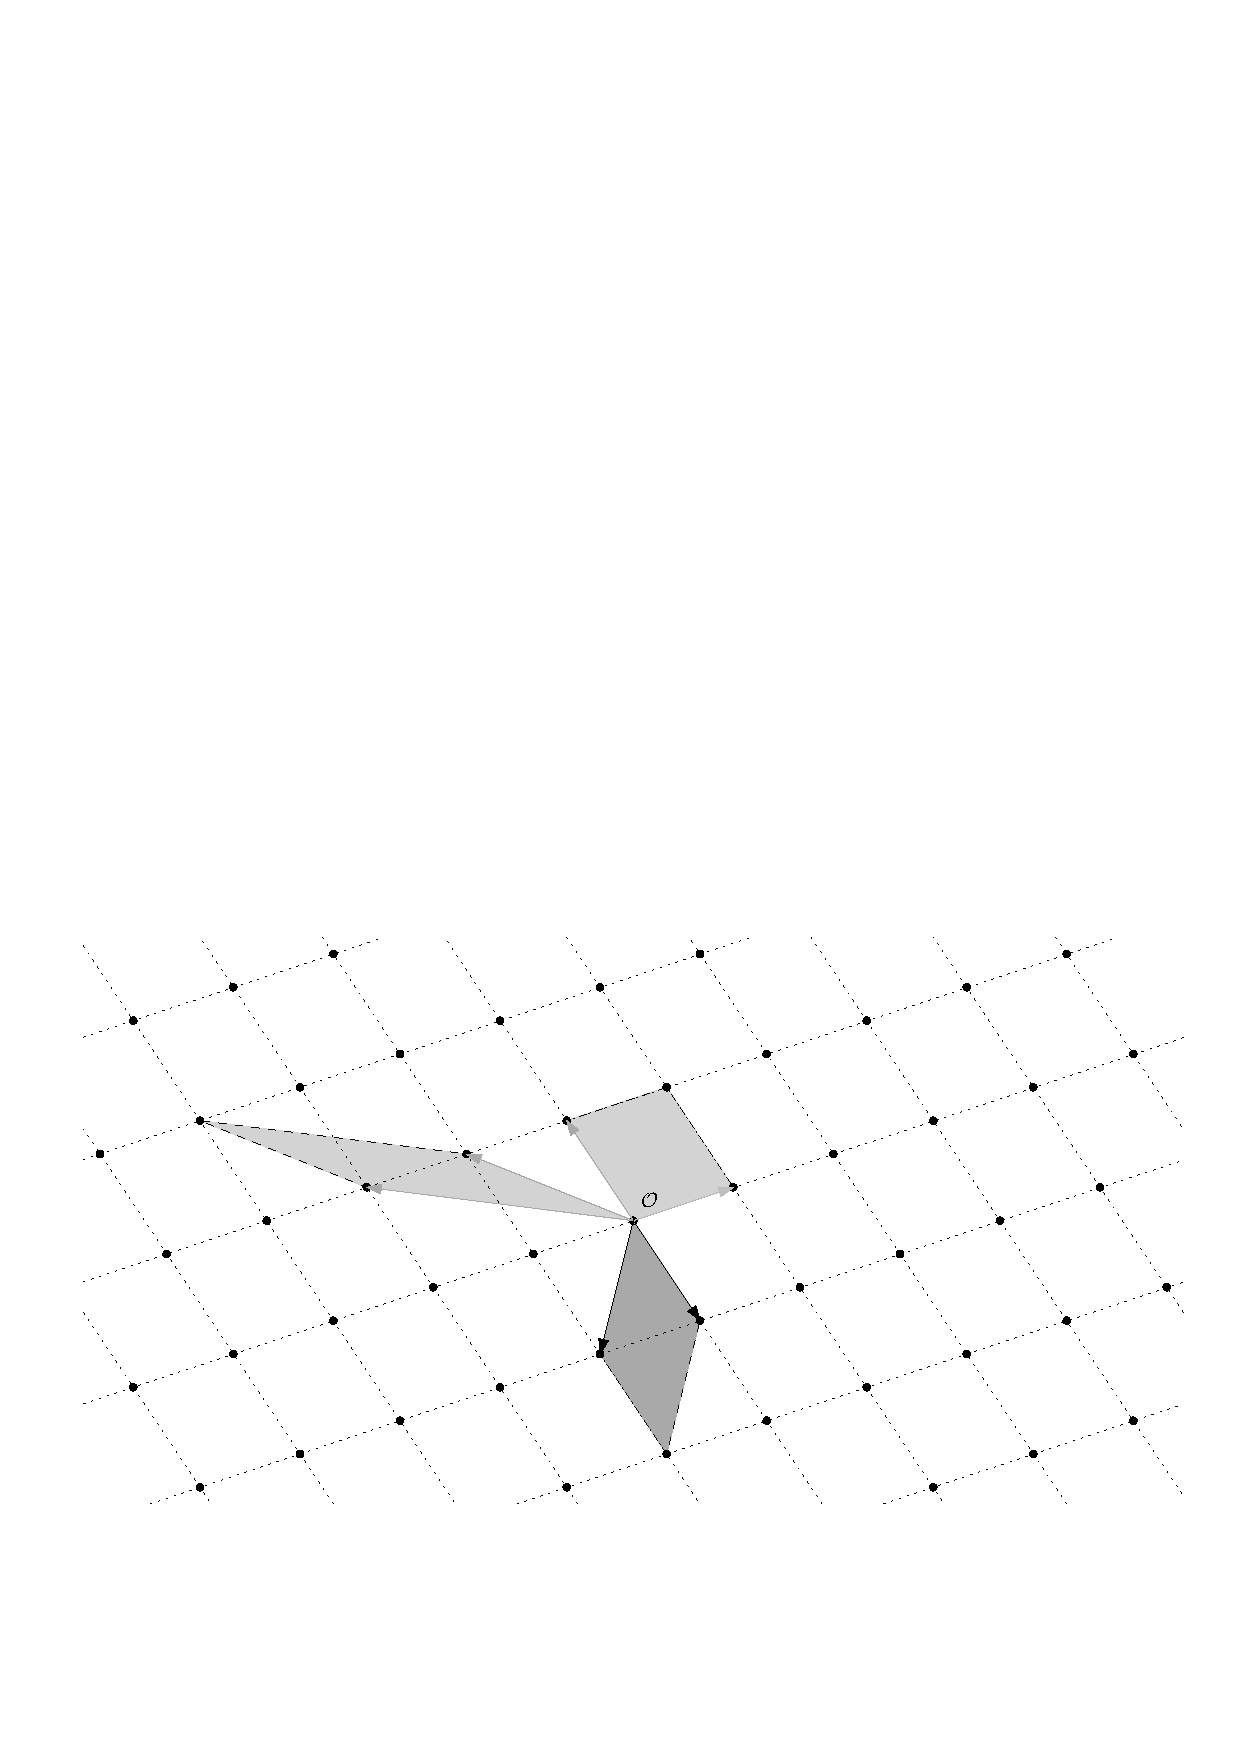
\includegraphics[width=0.8\linewidth]{./assets/lattice-volume.pdf}
\end{center}

\tiny Picture Credit: Joop van de Pol
\end{frame}

\begin{frame}[label={sec:orgb7b4454}]{Gaussian Heuristic}
\begin{itemize}
\item The Gaussian heuristic predicts that the number \(|\Lambda \cap \mathcal{B}|\) of lattice points inside a measurable body \(\mathcal{B} \subset \RR^d\) is approximately equal to \(\Vol(\mathcal{B}) / \Vol(\Lambda)\).
\item Applied to Euclidean \(d\)-balls, this means that a shortest vector in a lattice has expected norm \[λ_1(Λ) ≈ \textnormal{GH}(d) \cdot \mathsf{Vol}(\Lambda)^{1/d} \approx \sqrt{\frac{d}{2 π e}} \cdot \mathsf{Vol}(\Lambda)^{1/d} .\]
\end{itemize}

\begin{block}{Unusually Shortest Vector}
When \(λ_1(Λ) \ll \sqrt{\frac{d}{2 π e}} \cdot \mathsf{Vol}(\Lambda)^{1/d}\).
\end{block}
\end{frame}

\begin{frame}[label={sec:orge7ce25d}]{Length of Gram--Schmidt Vectors}
It will be useful to consider the lengths of the Gram--Schmidt vectors.

The vector \(\vec{b}^*_i\) is the orthogonal projection of \(\vec{b}_i\) to the space spanned by the vectors \(\vec{b}_0, \ldots, \vec{b}_{i-1}\).

\begin{columns}
\begin{column}{0.45\columnwidth}
\vspace{1em}

Informally, this means taking out the contributions in the directions of previous vectors  \(\vec{b}_0, \ldots, \vec{b}_{i-1}\).

\vspace{1em}

We have \(\Vol(\Lambda) = \prod_{i=0}^{d-1} \|\vec{b}_{i}^{*}\|\).
\end{column}

\begin{column}{0.45\columnwidth}
\begin{tikzpicture}
\pgfplotsset{width=\textwidth, height=0.6\textwidth}
\draw[->] (0,0) -- (3,1);
\node[] at (3.2,1.2) {$\vec{b}_0$};
\only<1>{\draw[->] (0,0) -- (1,2);}
\only<1>{\node[] at (1.2,2.2) {$\vec{b}_1$};}
\only<2>{\draw[->,color=lightgray] (0,0) -- (1,2);}
\only<2>{\node[color=lightgray] at (1.2,2.2) {$\vec{b}_1$};}
\only<2>{\draw[->,gray] (0,0) -- (-0.5,1.5);}
\only<2>{\node[] at (-0.3,1.7) {$\vec{b}^*_1$};}
\only<1>{\node[] at (-0.3,1.7) {\phantom{$\vec{b}^*_1$}};}
\end{tikzpicture}
\end{column}
\end{columns}
\end{frame}

\begin{frame}[label={sec:orgcbd8949},fragile]{Example}
 \lstset{language=Python,label= ,caption= ,captionpos=b,numbers=none}
\begin{lstlisting}
A = IntegerMatrix.random(120, "qary", k=60, bits=20)[::-1]
M = GSO.Mat(A, update=True)
line([(i,log(r_, 2)/2) for i, r_ in enumerate(M.r())], **plot_kwds)
\end{lstlisting}

\begin{center}
\includegraphics[width=.9\linewidth]{cache/log-gso-input.png}
\end{center}
\end{frame}

\begin{frame}[label={sec:orgeb966be},fragile]{Example - LLL}
 \lstset{language=Python,label= ,caption= ,captionpos=b,numbers=none}
\begin{lstlisting}
A = LLL.reduction(A)
M = GSO.Mat(A, update=True)
line([(i,log(r_, 2)/2) for i, r_ in enumerate(M.r())], **plot_kwds)
\end{lstlisting}

\begin{center}
\includegraphics[width=.9\linewidth]{./cache/log-gso-lll.png}
\end{center}
\end{frame}

\begin{frame}[label={sec:orgfaeec74}]{GSA}
\begin{center}
\includegraphics[width=.9\linewidth]{cache/log-gso-bkz-40.png}
\end{center}

\textbf{Geometric Series Assumption:} The shape after lattice reduction is a line with a flatter slope as lattice reduction gets stronger.\footfullcite{STACS:Schnorr03}
\end{frame}

\begin{frame}[label={sec:org4bd7f74}]{Strong Lattice Reduction: BKZ Algorithm (Block 0)}
\centering
\(\left(\begin{array}{ccccccccc}
\phantom{\pi_0(\vec{b}_0)} &
\phantom{\pi_0(\vec{b}_1)} &
\phantom{\pi_0(\vec{b}_2)} &
\phantom{\pi_0(\vec{b}_3)} &
\phantom{\pi_0(\vec{b}_4)} &
\phantom{\pi_0(\vec{b}_5)} &
\phantom{\pi_0(\vec{b}_6)} &
\phantom{\pi_0(\vec{b}_7)} & 
\\
\\
\\
\only<1-2>{\vec{b}_{0}}\only<3->{{\color{LightRed}\vec{b}_{0}}} &
          {\vec{b}_{1}}                                         &
          {\vec{b}_{2}}                                         &
          {\vec{b}_{3}}                                         &
          {\vec{b}_{4}}                                         &
          {\vec{b}_{5}}                                         &
          {\vec{b}_{6}}                                         &
          {\vec{b}_{7}}                                         &
\ldots\\
\\
\\
\\
\end{array}\right)\)
\begin{tikzpicture}[remember picture, overlay]
\tikzset{shift={(current page.center)},yshift=-1.5cm}
\node[] at (0,0) (origin) {};
{\color{DarkBlue} %
  \draw (-5.1,3.0) -- (-5.1,2.0) {};
  \draw (-5.1,1.0) -- (-5.1,0.0) {};
  \draw (0.2,3.0) -- (0.2,2.0) {};
  \draw (0.2,1.0) -- (0.2,0.0) {};
  \draw[decorate,decoration={brace,amplitude=10pt}] (-5.1,3.2) -- (0.2,3.2) node [black,midway,yshift=.6cm]{$\beta = 5$};
  \only<2>{%
    \draw[decorate,decoration={brace,amplitude=10pt}] (0.2,-0.2) -- (-5.1,-0.2) {};
  }
}
\node (oracle) at (-3,-1.8) {
\includegraphics[scale=0.9]{./assets/oracle.png}};
\only<2>{%
  \draw[->] (-4.5,-.8) .. controls (-4.3,-1.4) and (-3.8,-1.6)  .. (-3.5,-1.8);
  \draw[->] (-2.5,-1.8) .. controls (-2.3,-1.7)  and (-2.0,-1.6).. (-2.4,-.8);
}
\node at (5, -2.5) {\tiny{Picture credit: Eamonn Postlethwaite}};
\end{tikzpicture}
\end{frame}

\begin{frame}[label={sec:orgfc0f0a5}]{Strong Lattice Reduction: BKZ Algorithm (Block 1)}
\centering
\(\left(\begin{array}{ccccccccc}
\phantom{\pi_0(\vec{b}_0)} &
\phantom{\pi_0(\vec{b}_1)} &
\phantom{\pi_0(\vec{b}_2)} &
\phantom{\pi_0(\vec{b}_3)} &
\phantom{\pi_0(\vec{b}_4)} &
\phantom{\pi_0(\vec{b}_5)} &
\phantom{\pi_0(\vec{b}_6)} &
\phantom{\pi_0(\vec{b}_7)} & 
\\
\\
\\
{\color{LightRed}\vec{b}_{0}}                                               &
\only<1-2>{\pi_0(\vec{b}_{1})}\only<3->{{\color{LightRed}\pi_{0}(\vec{b}_{1})}} &
          {\pi_0(\vec{b}_{2})}                                                &
          {\pi_0(\vec{b}_{3})}                                                &
          {\pi_0(\vec{b}_{4})}                                                &
          {\pi_0(\vec{b}_{5})}                                                &
          {\vec{b}_{6}}                                                     &
          {\vec{b}_{7}}                                                     &
\ldots\\
\\
\\
\\
\end{array}\right)\)
\begin{tikzpicture}[remember picture, overlay]
\tikzset{shift={(current page.center)},yshift=-1.5cm}
\node[] at (0,0) (origin) {};
{\color{DarkBlue} %
  \draw (-3.8,3.0) -- (-3.8,2.0) {};
  \draw (-3.8,1.0) -- (-3.8,0.0) {};
  \draw (1.4,3.0) -- (1.4,2.0) {};
  \draw (1.4,1.0) -- (1.4,0.0) {};
  \draw[decorate,decoration={brace,amplitude=10pt}] (-3.8,3.2) -- (1.4,3.2) node [black,midway,yshift=.6cm]{$\beta = 5$};
  \only<2>{%
    \draw[decorate,decoration={brace,amplitude=10pt}] (1.4,-0.2) -- (-3.8,-0.2) {};
  }
}
\node (oracle) at (-3,-1.8) {
\includegraphics[scale=0.9]{./assets/oracle.png}};
\only<2>{%
  \draw[->] (-3.8,-.8) .. controls (-3.7,-1.6) and (-3.6,-1.6)  .. (-3.5,-1.8);
  \draw[->] (-2.5,-1.8) .. controls (-2.0,-1.7)  and (-1.4,-1.6).. (-1.2,-.8);
}
\node at (2.5, -2) {\(\pi_{i}(\vec{v})\): project \(\vec{v}\) orthogonally to \(\vec{b}_{0}, \ldots, \vec{b}_{i}\)};
\end{tikzpicture}
\end{frame}

\begin{frame}[label={sec:org8aebe50}]{BKZ Algorithm}
\begin{algorithm}[H]
  \KwData{LLL-reduced lattice basis \(\mat{B}\)}
  \KwData{block size \(\beta\)}
  \SetKwFor{MRepeat}{repeat}{}{}
  \MRepeat{until no more change}{
    \For{\(\kappa \gets 0\) \KwTo{} \(d-1\)}{
        LLL  on local projected block \([\kappa,\ldots,\kappa+\beta-1]\)\; 
        \(\vec{v} \gets \) find shortest vector in local projected block \([\kappa,\ldots,\kappa+\beta-1]\)\;
        insert $\vec{v}$ into $\vec{B}$\;
    }
  }
\end{algorithm}
\end{frame}

\begin{frame}[label={sec:orgaeccc83},fragile]{Quality}
 \centering
\begin{tabular}{l@{\hskip 4em}l}
For SIS & For BDD \\
$\|\vec{b}_{0}\| \approx {\delta_{\beta}}^{{d-1}} \cdot {\Vol(\Lambda)}^{1/d}$ & $\|\vec b_{0}\| \approx {\delta_{\beta}}^{2\cdot{(d-\beta)}} \cdot \lambda_{1}(\Lambda)$\\
\end{tabular}

\begin{center}
\begin{tabular}{rrrrrrrr}
\toprule
\(\beta\) & 2 & 5 & 24 & 50 & 100 & 200 & 500\\
\midrule
\(\delta\)\textsubscript{\(\beta\)} & 1.0219 & 1.0186 & 1.0142 & 1.0121 & 1.0096 & 1.0063 & 1.0034\\
\bottomrule
\end{tabular}

\end{center}

\begin{itemize}
\item We have \textbf{Root Hermite Factor} \(\delta_{\beta} \approx \GH(\beta)^{1/(\beta-1)}\) for \(\beta > 50\).

\lstset{language=Python,label= ,caption= ,captionpos=b,numbers=none}
\begin{lstlisting}
RC.delta(500)
\end{lstlisting}

\begin{verbatim}
1.00340402678510
\end{verbatim}

\item The slope under the \textbf{Geometric Series Assumption} is \(\alpha_{\beta} = \delta_{\beta}^{-2}\).
\end{itemize}
\end{frame}

\begin{frame}[allowframebreaks]{Behaviour in Practice: BKZ-60 in Dimension 180}
\tikzset{external/export=true}

\vspace{-0.8em}
\tikzsetnextfilename{bkz-loggso-evolution0-lll}
\begin{tikzpicture}
  \begin{axis}[ylabel=\(\log_2(\|\vec{b}_i^*\|)\),xlabel=\(i\),legend pos=north east,height=0.5\textwidth,ymin=3,ymax=16,xmin=0,xmax=180]
    \addplot+[black] table [x=i, y=gsa, col sep=comma]{data/bkz-60-180-loggso-evolution.csv};
    \addlegendentry{GSA};
    \addplot+[] table [x=i, y=lll, col sep=comma]{data/bkz-60-180-loggso-evolution.csv};
    \addlegendentry{LLL};
  \end{axis}
\end{tikzpicture}

\framebreak

\tikzsetnextfilename{bkz-loggso-evolution1}
\begin{tikzpicture}
  \begin{axis}[ylabel=\(\log_2(\|\vec{b}_i^*\|)\),xlabel=\(i\),legend pos=north east,height=0.5\textwidth,ymin=3,ymax=16,xmin=0,xmax=180]
    \addplot+[black] table [x=i, y=gsa, col sep=comma]{data/bkz-60-180-loggso-evolution.csv};
    \addlegendentry{GSA};
    \addplot+[] table [x=i, y=tour0, col sep=comma]{data/bkz-60-180-loggso-evolution.csv};
    \addlegendentry{Tour 0};
  \end{axis}
\end{tikzpicture}

\framebreak

\tikzsetnextfilename{bkz-loggso-evolution2}
\begin{tikzpicture}
  \begin{axis}[ylabel=\(\log_2(\|\vec{b}_i^*\|)\),xlabel=\(i\),legend pos=north east,height=0.5\textwidth,ymin=3,ymax=16,xmin=0,xmax=180]
    \addplot+[black] table [x=i, y=gsa, col sep=comma]{data/bkz-60-180-loggso-evolution.csv};
    \addlegendentry{GSA};
    \addplot+[] table [x=i, y=tour1, col sep=comma]{data/bkz-60-180-loggso-evolution.csv};
    \addlegendentry{Tour 1};
  \end{axis}
\end{tikzpicture}


\framebreak

\tikzsetnextfilename{bkz-loggso-evolution3}
\begin{tikzpicture}
  \begin{axis}[ylabel=\(\log_2(\|\vec{b}_i^*\|)\),xlabel=\(i\),legend pos=north east,height=0.5\textwidth,ymin=3,ymax=16,xmin=0,xmax=180]
    \addplot+[black] table [x=i, y=gsa, col sep=comma]{data/bkz-60-180-loggso-evolution.csv};
    \addlegendentry{GSA};
    \addplot+[] table [x=i, y=tour2, col sep=comma]{data/bkz-60-180-loggso-evolution.csv};
    \addlegendentry{Tour 2};
  \end{axis}
\end{tikzpicture}

\framebreak

\tikzsetnextfilename{bkz-loggso-evolution4}
\begin{tikzpicture}
  \begin{axis}[ylabel=\(\log_2(\|\vec{b}_i^*\|)\),xlabel=\(i\),legend pos=north east,height=0.5\textwidth,ymin=3,ymax=16,xmin=0,xmax=180]
    \addplot+[black] table [x=i, y=gsa, col sep=comma]{data/bkz-60-180-loggso-evolution.csv};
    \addlegendentry{GSA};
    \addplot+[] table [x=i, y=tour3, col sep=comma]{data/bkz-60-180-loggso-evolution.csv};
    \addlegendentry{Tour 3};
  \end{axis}
\end{tikzpicture}

\framebreak

\tikzsetnextfilename{bkz-loggso-evolution5}
\begin{tikzpicture}
  \begin{axis}[ylabel=\(\log_2(\|\vec{b}_i^*\|)\),xlabel=\(i\),legend pos=north east,height=0.5\textwidth,ymin=3,ymax=16,xmin=0,xmax=180]
    \addplot+[black] table [x=i, y=gsa, col sep=comma]{data/bkz-60-180-loggso-evolution.csv};
    \addlegendentry{GSA};
    \addplot+[] table [x=i, y=tour4, col sep=comma]{data/bkz-60-180-loggso-evolution.csv};
    \addlegendentry{Tour 4};
  \end{axis}
\end{tikzpicture}

\framebreak

\tikzsetnextfilename{bkz-loggso-evolution6}
\begin{tikzpicture}
  \begin{axis}[ylabel=\(\log_2(\|\vec{b}_i^*\|)\),xlabel=\(i\),legend pos=north east,height=0.5\textwidth,ymin=3,ymax=16,xmin=0,xmax=180]
    \addplot+[black] table [x=i, y=gsa, col sep=comma]{data/bkz-60-180-loggso-evolution.csv};
    \addlegendentry{GSA};
    \addplot+[] table [x=i, y=tour5, col sep=comma]{data/bkz-60-180-loggso-evolution.csv};
    \addlegendentry{Tour 5};
  \end{axis}
\end{tikzpicture}

\framebreak

\tikzsetnextfilename{bkz-loggso-evolution7}
\begin{tikzpicture}
  \begin{axis}[ylabel=\(\log_2(\|\vec{b}_i^*\|)\),xlabel=\(i\),legend pos=north east,height=0.5\textwidth,ymin=3,ymax=16,xmin=0,xmax=180]
    \addplot+[black] table [x=i, y=gsa, col sep=comma]{data/bkz-60-180-loggso-evolution.csv};
    \addlegendentry{GSA};
    \addplot+[] table [x=i, y=tour6, col sep=comma]{data/bkz-60-180-loggso-evolution.csv};
    \addlegendentry{Tour 6};
  \end{axis}
\end{tikzpicture}

\framebreak

\tikzsetnextfilename{bkz-loggso-evolution8}
\begin{tikzpicture}
  \begin{axis}[ylabel=\(\log_2(\|\vec{b}_i^*\|)\),xlabel=\(i\),legend pos=north east,height=0.5\textwidth,ymin=3,ymax=16,xmin=0,xmax=180]
    \addplot+[black] table [x=i, y=gsa, col sep=comma]{data/bkz-60-180-loggso-evolution.csv};
    \addlegendentry{GSA};
    \addplot+[] table [x=i, y=tour7, col sep=comma]{data/bkz-60-180-loggso-evolution.csv};
    \addlegendentry{Tour 7};
  \end{axis}
\end{tikzpicture}


\framebreak

\tikzsetnextfilename{bkz-loggso-evolution9}
\begin{tikzpicture}
  \begin{axis}[ylabel=\(\log_2(\|\vec{b}_i^*\|)\),xlabel=\(i\),legend pos=north east,height=0.5\textwidth,ymin=3,ymax=16,xmin=0,xmax=180]
    \addplot+[black] table [x=i, y=simulator, col sep=comma]{data/bkz-60-180-loggso-evolution.csv};
    \addlegendentry{Simulator};
    \addplot+[] table [x=i, y=tour7, col sep=comma]{data/bkz-60-180-loggso-evolution.csv};
    \addlegendentry{Tour 7};
  \end{axis}
\end{tikzpicture}

\tikzset{external/export=false}
\end{frame}

\begin{frame}[label={sec:org19978ba},fragile]{Try it at Home}
 \lstset{language=Python,label= ,caption= ,captionpos=b,numbers=none}
\begin{lstlisting}
from fpylll import *
from fpylll.algorithms.bkz2 import BKZReduction as BKZ2
A = IntegerMatrix.random(180, "qary", k=90, bits=20)
bkz = BKZ2(A)
bkz(BKZ.EasyParam(block_size=60))
\end{lstlisting}

\begin{description}
\item[{\url{https://github.com/fplll/fplll}}] C++ library
\item[{\url{https://github.com/fplll/fpylll}}] Python interface
\item[{\url{https://github.com/fplll/g6k}}] Sieving (faster lattice reduction)
\item[{\url{https://sagemath.org}}] FPyLLL is in SageMath
\item[{\url{https://sagecell.sagemath.org/}}] SageMath in your browser
\item[{\url{https://cocalc.com/}}] SageMath worksheets in your browser
\end{description}
\end{frame}

\begin{frame}[label={sec:org03f6f3f}]{Success Condition for uSVP (Expectation)}
%\vspace{-2.6em}

\tikzset{external/export=true}
\tikzsetnextfilename{usvp-success-expectation}
\begin{tikzpicture}
\begin{axis}[/pgf/number format/.cd,fixed,ymin = 1,legend pos=north east,legend style={fill=white}, xlabel=,ylabel=$\log_2(\norm \cdot)$,width=\columnwidth, height=0.4\columnwidth, xmin = 1, xmax = 183,legend cell align=left,ymax=9]
%      \draw[->] (-3,0) -- (4.2,0) node[right] {$x$};
%      \draw[->] (0,-3) -- (0,4.2) node[above] {$y$};
\addplot[domain=1:183,smooth,variable=\x,black] plot ({\x},{log2(1.01170246711949^(-2*(\x-1)+183)*54.5751087741536)});
\addlegendentry{GSA for $\norm{\vec b_i^*}$}

\addplot[domain=1:183,samples=1000, smooth,variable=\x,darkgray,dotted,thick] plot ({\x},{log2( 3.19153824321146 * sqrt(183 - \x + 1) )});

\addlegendentry{length of projection of $(\vec{e},\vec{s},1)$}

\draw[dashed] (127,1) -- (127,820) node[pos = 0.06, right] {$d-\beta$};
\end{axis}
\end{tikzpicture}
\tikzset{external/export=false}

\vspace{-1.3em}
\[\sqrt{\beta/d} \cdot \sigma \leq {\delta_{\beta}}^{2\beta-d-1} \cdot \Vol(\Lambda)^{1/d}\]

\scriptsize{

\fullcite{USENIX:ADPS16}  \phantom{Foo Foo Foo Foo Foo Foo Foo Foo Foo Foo Foo Foo Foo}

}
\end{frame}

\begin{frame}[label={sec:org2a963cb}]{Success Condition for uSVP (Observed)}
\tikzset{external/export=true}
\tikzsetnextfilename{usv-success-observation}
\begin{tikzpicture}
\begin{axis}[/pgf/number format/.cd,fixed, ymin = 1,legend pos=north east, xlabel= ,ylabel=$\log_2(\norm \cdot)$,width=\columnwidth, height=0.4\columnwidth, xmin = 1, xmax = 183,legend cell align=left,ymax=9]
%      \draw[->] (-3,0) -- (4.2,0) node[right] {$x$};
%      \draw[->] (0,-3) -- (0,4.2) node[above] {$y$};

\addplot[gray,thick,x filter/.code={\pgfmathparse{\pgfmathresult+1.0}}] coordinates {
   (  0,  8.78) (  1,  8.78) (  2,  8.77) (  3,  8.72) (  4,  8.71) (  5,  8.69) (  6,  8.66) (  7,  8.63) (  8,  8.62) (  9,  8.59) ( 10,  8.54) ( 11,  8.53) ( 12,  8.51) ( 13,  8.47) ( 14,  8.43) ( 15,  8.39) ( 16,  8.36) ( 17,  8.34) ( 18,  8.30) ( 19,  8.28) ( 20,  8.24) ( 21,  8.20) ( 22,  8.16) ( 23,  8.13) ( 24,  8.10) ( 25,  8.07) ( 26,  8.04) ( 27,  7.99) ( 28,  7.96) ( 29,  7.94) ( 30,  7.91) ( 31,  7.88) ( 32,  7.84) ( 33,  7.79) ( 34,  7.76) ( 35,  7.73) ( 36,  7.69) ( 37,  7.65) ( 38,  7.61) ( 39,  7.59) ( 40,  7.55) ( 41,  7.52) ( 42,  7.48) ( 43,  7.44) ( 44,  7.39) ( 45,  7.37) ( 46,  7.33) ( 47,  7.31) ( 48,  7.27) ( 49,  7.24) ( 50,  7.21) ( 51,  7.18) ( 52,  7.15) ( 53,  7.09) ( 54,  7.07) ( 55,  7.03) ( 56,  7.00) ( 57,  6.97) ( 58,  6.95) ( 59,  6.91) ( 60,  6.87) ( 61,  6.83) ( 62,  6.79) ( 63,  6.74) ( 64,  6.72) ( 65,  6.67) ( 66,  6.64) ( 67,  6.62) ( 68,  6.59) ( 69,  6.55) ( 70,  6.52) ( 71,  6.46) ( 72,  6.44) ( 73,  6.40) ( 74,  6.38) ( 75,  6.34) ( 76,  6.31) ( 77,  6.28) ( 78,  6.24) ( 79,  6.21) ( 80,  6.15) ( 81,  6.13) ( 82,  6.09) ( 83,  6.06) ( 84,  6.02) ( 85,  6.00) ( 86,  5.97) ( 87,  5.92) ( 88,  5.88) ( 89,  5.86) ( 90,  5.82) ( 91,  5.78) ( 92,  5.75) ( 93,  5.73) ( 94,  5.71) ( 95,  5.66) ( 96,  5.64) ( 97,  5.59) ( 98,  5.55) ( 99,  5.51) (100,  5.47) (101,  5.43) (102,  5.41) (103,  5.36) (104,  5.36) (105,  5.31) (106,  5.28) (107,  5.25) (108,  5.23) (109,  5.18) (110,  5.13) (111,  5.09) (112,  5.04) (113,  5.01) (114,  5.00) (115,  4.96) (116,  4.92) (117,  4.86) (118,  4.83) (119,  4.79) (120,  4.77) (121,  4.72) (122,  4.68) (123,  4.66) (124,  4.63) (125,  4.60) (126,  4.56) (127,  4.52) (128,  4.50) (129,  4.45) (130,  4.43) (131,  4.40) (132,  4.36) (133,  4.34) (134,  4.30) (135,  4.27) (136,  4.24) (137,  4.22) (138,  4.18) (139,  4.16) (140,  4.12) (141,  4.09) (142,  4.06) (143,  4.03) (144,  4.01) (145,  3.95) (146,  3.91) (147,  3.89) (148,  3.85) (149,  3.81) (150,  3.77) (151,  3.75) (152,  3.71) (153,  3.66) (154,  3.62) (155,  3.59) (156,  3.55) (157,  3.51) (158,  3.47) (159,  3.43) (160,  3.39) (161,  3.37) (162,  3.29) (163,  3.27) (164,  3.23) (165,  3.19) (166,  3.13) (167,  3.08) (168,  3.03) (169,  2.99) (170,  2.94) (171,  2.89) (172,  2.84) (173,  2.79) (174,  2.76) (175,  2.72) (176,  2.68) (177,  2.65) (178,  2.61) (179,  2.58) (180,  2.51) (181,  2.54) (182,  2.56) };
\addlegendentry{Average for $\norm{\vec b_i^*}$}

  \addplot[black] coordinates {(  1, 5.453) (  2, 5.450) (  3, 5.449) (  4, 5.446) (  5, 5.442) (  6, 5.434) (  7, 5.430) (  8, 5.428) (  9, 5.424) ( 10, 5.416) ( 11, 5.411) ( 12, 5.407) ( 13, 5.402) ( 14, 5.397) ( 15, 5.392) ( 16, 5.388) ( 17, 5.385) ( 18, 5.383) ( 19, 5.380) ( 20, 5.375) ( 21, 5.366) ( 22, 5.358) ( 23, 5.355) ( 24, 5.352) ( 25, 5.350) ( 26, 5.345) ( 27, 5.341) ( 28, 5.336) ( 29, 5.332) ( 30, 5.327) ( 31, 5.322) ( 32, 5.317) ( 33, 5.312) ( 34, 5.307) ( 35, 5.305) ( 36, 5.299) ( 37, 5.296) ( 38, 5.290) ( 39, 5.285) ( 40, 5.279) ( 41, 5.276) ( 42, 5.273) ( 43, 5.267) ( 44, 5.261) ( 45, 5.255) ( 46, 5.252) ( 47, 5.248) ( 48, 5.241) ( 49, 5.237) ( 50, 5.233) ( 51, 5.230) ( 52, 5.222) ( 53, 5.217) ( 54, 5.209) ( 55, 5.206) ( 56, 5.204) ( 57, 5.197) ( 58, 5.190) ( 59, 5.182) ( 60, 5.175) ( 61, 5.166) ( 62, 5.157) ( 63, 5.151) ( 64, 5.144) ( 65, 5.139) ( 66, 5.132) ( 67, 5.123) ( 68, 5.117) ( 69, 5.111) ( 70, 5.108) ( 71, 5.105) ( 72, 5.099) ( 73, 5.087) ( 74, 5.082) ( 75, 5.078) ( 76, 5.074) ( 77, 5.063) ( 78, 5.057) ( 79, 5.052) ( 80, 5.041) ( 81, 5.026) ( 82, 5.021) ( 83, 5.013) ( 84, 5.001) ( 85, 4.996) ( 86, 4.988) ( 87, 4.970) ( 88, 4.963) ( 89, 4.956) ( 90, 4.949) ( 91, 4.941) ( 92, 4.937) ( 93, 4.929) ( 94, 4.925) ( 95, 4.915) ( 96, 4.909) ( 97, 4.898) ( 98, 4.887) ( 99, 4.875) (100, 4.860) (101, 4.846) (102, 4.830) (103, 4.824) (104, 4.815) (105, 4.806) (106, 4.796) (107, 4.791) (108, 4.780) (109, 4.759) (110, 4.750) (111, 4.741) (112, 4.729) (113, 4.714) (114, 4.699) (115, 4.685) (116, 4.680) (117, 4.668) (118, 4.659) (119, 4.651) (120, 4.641) (121, 4.628) (122, 4.619) (123, 4.605) (124, 4.590) (125, 4.577) (126, 4.567) (127, 4.558) (128, 4.545) (129, 4.537) (130, 4.525) (131, 4.506) (132, 4.489) (133, 4.480) (134, 4.471) (135, 4.459) (136, 4.443) (137, 4.424) (138, 4.412) (139, 4.404) (140, 4.392) (141, 4.374) (142, 4.363) (143, 4.342) (144, 4.316) (145, 4.291) (146, 4.268) (147, 4.242) (148, 4.221) (149, 4.198) (150, 4.174) (151, 4.128) (152, 4.088) (153, 4.073) (154, 4.041) (155, 4.024) (156, 4.006) (157, 3.972) (158, 3.952) (159, 3.929) (160, 3.896) (161, 3.875) (162, 3.797) (163, 3.744) (164, 3.702) (165, 3.675) (166, 3.643) (167, 3.592) (168, 3.552) (169, 3.515) (170, 3.455) (171, 3.411) (172, 3.367) (173, 3.313) (174, 3.246) (175, 3.188) (176, 3.054) (177, 2.936) (178, 2.866) (179, 2.704) (180, 2.464) (181, 2.141) (182, 1.682)};
\addlegendentry{Average for $\norm{\pi_i(\vec e,\vec s,1)}$}

\draw[dashed] (127,1) -- (127,820) node[pos = 0.06, right] {$d-\beta$};
\end{axis}
\end{tikzpicture}
\tikzset{external/export=false}

\scriptsize{

\fullcite{AC:AGVW17}

\fullcite{PKC:PosVir21}

}
\end{frame}

\begin{frame}[label={sec:org7135eb5}]{The GSA is a Lie: Tail Shape}
\tikzset{external/export=true}
\tikzsetnextfilename{gsa-comparison}
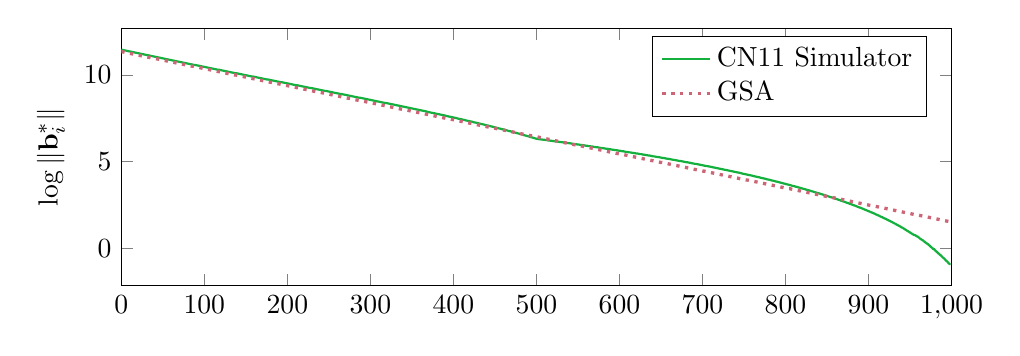
\begin{tikzpicture}
\begin{axis}[xmin=0,xmax=1000,ylabel=\(\log \|\vec{b}_{i}^{*}\|\),legend pos=north east,height=0.4\textwidth]
\addplot+[] coordinates {
(  0, 11.45) (  1, 11.44) (  2, 11.43) (  3, 11.42) (  4, 11.41) (  5, 11.40) (  6, 11.39) 
(  7, 11.38) (  8, 11.37) (  9, 11.36) ( 10, 11.35) ( 11, 11.34) ( 12, 11.33) ( 13, 11.32) 
( 14, 11.31) ( 15, 11.30) ( 16, 11.29) ( 17, 11.28) ( 18, 11.27) ( 19, 11.26) ( 20, 11.25) 
( 21, 11.24) ( 22, 11.23) ( 23, 11.22) ( 24, 11.21) ( 25, 11.20) ( 26, 11.19) ( 27, 11.18) 
( 28, 11.17) ( 29, 11.16) ( 30, 11.15) ( 31, 11.14) ( 32, 11.13) ( 33, 11.12) ( 34, 11.11) 
( 35, 11.10) ( 36, 11.09) ( 37, 11.08) ( 38, 11.07) ( 39, 11.06) ( 40, 11.05) ( 41, 11.04) 
( 42, 11.03) ( 43, 11.02) ( 44, 11.01) ( 45, 11.00) ( 46, 10.99) ( 47, 10.98) ( 48, 10.97) 
( 49, 10.96) ( 50, 10.95) ( 51, 10.94) ( 52, 10.93) ( 53, 10.92) ( 54, 10.91) ( 55, 10.90) 
( 56, 10.89) ( 57, 10.88) ( 58, 10.87) ( 59, 10.86) ( 60, 10.85) ( 61, 10.84) ( 62, 10.83) 
( 63, 10.82) ( 64, 10.81) ( 65, 10.80) ( 66, 10.79) ( 67, 10.78) ( 68, 10.77) ( 69, 10.76) 
( 70, 10.75) ( 71, 10.74) ( 72, 10.73) ( 73, 10.72) ( 74, 10.71) ( 75, 10.70) ( 76, 10.69) 
( 77, 10.68) ( 78, 10.67) ( 79, 10.66) ( 80, 10.65) ( 81, 10.64) ( 82, 10.63) ( 83, 10.62) 
( 84, 10.61) ( 85, 10.60) ( 86, 10.59) ( 87, 10.58) ( 88, 10.57) ( 89, 10.57) ( 90, 10.56) 
( 91, 10.55) ( 92, 10.54) ( 93, 10.53) ( 94, 10.52) ( 95, 10.51) ( 96, 10.50) ( 97, 10.49) 
( 98, 10.48) ( 99, 10.47) (100, 10.46) (101, 10.45) (102, 10.44) (103, 10.43) (104, 10.42) 
(105, 10.41) (106, 10.40) (107, 10.39) (108, 10.38) (109, 10.37) (110, 10.36) (111, 10.35) 
(112, 10.34) (113, 10.33) (114, 10.32) (115, 10.31) (116, 10.30) (117, 10.30) (118, 10.29) 
(119, 10.28) (120, 10.27) (121, 10.26) (122, 10.25) (123, 10.24) (124, 10.23) (125, 10.22) 
(126, 10.21) (127, 10.20) (128, 10.19) (129, 10.18) (130, 10.17) (131, 10.16) (132, 10.15) 
(133, 10.14) (134, 10.13) (135, 10.12) (136, 10.11) (137, 10.10) (138, 10.09) (139, 10.09) 
(140, 10.08) (141, 10.07) (142, 10.06) (143, 10.05) (144, 10.04) (145, 10.03) (146, 10.02) 
(147, 10.01) (148, 10.00) (149,  9.99) (150,  9.98) (151,  9.97) (152,  9.96) (153,  9.95) 
(154,  9.94) (155,  9.93) (156,  9.92) (157,  9.91) (158,  9.91) (159,  9.90) (160,  9.89) 
(161,  9.88) (162,  9.87) (163,  9.86) (164,  9.85) (165,  9.84) (166,  9.83) (167,  9.82) 
(168,  9.81) (169,  9.80) (170,  9.79) (171,  9.78) (172,  9.77) (173,  9.76) (174,  9.75) 
(175,  9.74) (176,  9.73) (177,  9.73) (178,  9.72) (179,  9.71) (180,  9.70) (181,  9.69) 
(182,  9.68) (183,  9.67) (184,  9.66) (185,  9.65) (186,  9.64) (187,  9.63) (188,  9.62) 
(189,  9.61) (190,  9.60) (191,  9.59) (192,  9.58) (193,  9.57) (194,  9.57) (195,  9.56) 
(196,  9.55) (197,  9.54) (198,  9.53) (199,  9.52) (200,  9.51) (201,  9.50) (202,  9.49) 
(203,  9.48) (204,  9.47) (205,  9.46) (206,  9.45) (207,  9.44) (208,  9.43) (209,  9.42) 
(210,  9.41) (211,  9.41) (212,  9.40) (213,  9.39) (214,  9.38) (215,  9.37) (216,  9.36) 
(217,  9.35) (218,  9.34) (219,  9.33) (220,  9.32) (221,  9.31) (222,  9.30) (223,  9.29) 
(224,  9.28) (225,  9.27) (226,  9.26) (227,  9.25) (228,  9.25) (229,  9.24) (230,  9.23) 
(231,  9.22) (232,  9.21) (233,  9.20) (234,  9.19) (235,  9.18) (236,  9.17) (237,  9.16) 
(238,  9.15) (239,  9.14) (240,  9.13) (241,  9.12) (242,  9.11) (243,  9.10) (244,  9.09) 
(245,  9.08) (246,  9.08) (247,  9.07) (248,  9.06) (249,  9.05) (250,  9.04) (251,  9.03) 
(252,  9.02) (253,  9.01) (254,  9.00) (255,  8.99) (256,  8.98) (257,  8.97) (258,  8.96) 
(259,  8.95) (260,  8.94) (261,  8.93) (262,  8.92) (263,  8.91) (264,  8.90) (265,  8.90) 
(266,  8.89) (267,  8.88) (268,  8.87) (269,  8.86) (270,  8.85) (271,  8.84) (272,  8.83) 
(273,  8.82) (274,  8.81) (275,  8.80) (276,  8.79) (277,  8.78) (278,  8.77) (279,  8.76) 
(280,  8.75) (281,  8.74) (282,  8.73) (283,  8.72) (284,  8.71) (285,  8.70) (286,  8.69) 
(287,  8.68) (288,  8.68) (289,  8.67) (290,  8.66) (291,  8.65) (292,  8.64) (293,  8.63) 
(294,  8.62) (295,  8.61) (296,  8.60) (297,  8.59) (298,  8.58) (299,  8.57) (300,  8.56) 
(301,  8.55) (302,  8.54) (303,  8.53) (304,  8.52) (305,  8.51) (306,  8.50) (307,  8.49) 
(308,  8.48) (309,  8.47) (310,  8.46) (311,  8.45) (312,  8.44) (313,  8.43) (314,  8.42) 
(315,  8.41) (316,  8.40) (317,  8.39) (318,  8.38) (319,  8.38) (320,  8.37) (321,  8.36) 
(322,  8.35) (323,  8.34) (324,  8.33) (325,  8.32) (326,  8.31) (327,  8.30) (328,  8.29) 
(329,  8.28) (330,  8.27) (331,  8.26) (332,  8.25) (333,  8.24) (334,  8.23) (335,  8.22) 
(336,  8.21) (337,  8.20) (338,  8.19) (339,  8.18) (340,  8.17) (341,  8.16) (342,  8.15) 
(343,  8.14) (344,  8.13) (345,  8.12) (346,  8.11) (347,  8.10) (348,  8.09) (349,  8.08) 
(350,  8.07) (351,  8.06) (352,  8.05) (353,  8.04) (354,  8.03) (355,  8.02) (356,  8.01) 
(357,  8.00) (358,  7.99) (359,  7.98) (360,  7.97) (361,  7.96) (362,  7.95) (363,  7.94) 
(364,  7.93) (365,  7.92) (366,  7.91) (367,  7.90) (368,  7.88) (369,  7.87) (370,  7.86) 
(371,  7.85) (372,  7.84) (373,  7.83) (374,  7.82) (375,  7.81) (376,  7.80) (377,  7.79) 
(378,  7.78) (379,  7.77) (380,  7.76) (381,  7.75) (382,  7.74) (383,  7.73) (384,  7.72) 
(385,  7.71) (386,  7.70) (387,  7.69) (388,  7.68) (389,  7.67) (390,  7.66) (391,  7.64) 
(392,  7.63) (393,  7.62) (394,  7.61) (395,  7.60) (396,  7.59) (397,  7.58) (398,  7.57) 
(399,  7.56) (400,  7.55) (401,  7.54) (402,  7.53) (403,  7.52) (404,  7.51) (405,  7.49) 
(406,  7.48) (407,  7.47) (408,  7.46) (409,  7.45) (410,  7.44) (411,  7.43) (412,  7.42) 
(413,  7.41) (414,  7.40) (415,  7.38) (416,  7.37) (417,  7.36) (418,  7.35) (419,  7.34) 
(420,  7.33) (421,  7.32) (422,  7.31) (423,  7.30) (424,  7.28) (425,  7.27) (426,  7.26) 
(427,  7.25) (428,  7.24) (429,  7.23) (430,  7.22) (431,  7.20) (432,  7.19) (433,  7.18) 
(434,  7.17) (435,  7.16) (436,  7.15) (437,  7.14) (438,  7.12) (439,  7.11) (440,  7.10) 
(441,  7.09) (442,  7.08) (443,  7.06) (444,  7.05) (445,  7.04) (446,  7.03) (447,  7.02) 
(448,  7.01) (449,  6.99) (450,  6.98) (451,  6.97) (452,  6.96) (453,  6.94) (454,  6.93) 
(455,  6.92) (456,  6.91) (457,  6.90) (458,  6.88) (459,  6.87) (460,  6.86) (461,  6.85) 
(462,  6.83) (463,  6.82) (464,  6.81) (465,  6.80) (466,  6.78) (467,  6.77) (468,  6.76) 
(469,  6.75) (470,  6.73) (471,  6.72) (472,  6.71) (473,  6.69) (474,  6.68) (475,  6.67) 
(476,  6.66) (477,  6.64) (478,  6.63) (479,  6.62) (480,  6.60) (481,  6.59) (482,  6.58) 
(483,  6.56) (484,  6.55) (485,  6.53) (486,  6.52) (487,  6.51) (488,  6.49) (489,  6.48) 
(490,  6.47) (491,  6.45) (492,  6.44) (493,  6.42) (494,  6.41) (495,  6.40) (496,  6.38) 
(497,  6.37) (498,  6.35) (499,  6.34) (500,  6.32) (501,  6.32) (502,  6.31) (503,  6.30) 
(504,  6.30) (505,  6.29) (506,  6.28) (507,  6.28) (508,  6.27) (509,  6.27) (510,  6.26) 
(511,  6.25) (512,  6.25) (513,  6.24) (514,  6.23) (515,  6.23) (516,  6.22) (517,  6.21) 
(518,  6.21) (519,  6.20) (520,  6.19) (521,  6.19) (522,  6.18) (523,  6.17) (524,  6.17) 
(525,  6.16) (526,  6.16) (527,  6.15) (528,  6.14) (529,  6.14) (530,  6.13) (531,  6.12) 
(532,  6.12) (533,  6.11) (534,  6.10) (535,  6.10) (536,  6.09) (537,  6.08) (538,  6.08) 
(539,  6.07) (540,  6.06) (541,  6.06) (542,  6.05) (543,  6.04) (544,  6.03) (545,  6.03) 
(546,  6.02) (547,  6.01) (548,  6.01) (549,  6.00) (550,  5.99) (551,  5.99) (552,  5.98) 
(553,  5.97) (554,  5.97) (555,  5.96) (556,  5.95) (557,  5.95) (558,  5.94) (559,  5.93) 
(560,  5.92) (561,  5.92) (562,  5.91) (563,  5.90) (564,  5.90) (565,  5.89) (566,  5.88) 
(567,  5.88) (568,  5.87) (569,  5.86) (570,  5.85) (571,  5.85) (572,  5.84) (573,  5.83) 
(574,  5.83) (575,  5.82) (576,  5.81) (577,  5.80) (578,  5.80) (579,  5.79) (580,  5.78) 
(581,  5.78) (582,  5.77) (583,  5.76) (584,  5.75) (585,  5.75) (586,  5.74) (587,  5.73) 
(588,  5.72) (589,  5.72) (590,  5.71) (591,  5.70) (592,  5.69) (593,  5.69) (594,  5.68) 
(595,  5.67) (596,  5.67) (597,  5.66) (598,  5.65) (599,  5.64) (600,  5.64) (601,  5.63) 
(602,  5.62) (603,  5.61) (604,  5.61) (605,  5.60) (606,  5.59) (607,  5.58) (608,  5.57) 
(609,  5.57) (610,  5.56) (611,  5.55) (612,  5.54) (613,  5.54) (614,  5.53) (615,  5.52) 
(616,  5.51) (617,  5.51) (618,  5.50) (619,  5.49) (620,  5.48) (621,  5.47) (622,  5.47) 
(623,  5.46) (624,  5.45) (625,  5.44) (626,  5.44) (627,  5.43) (628,  5.42) (629,  5.41) 
(630,  5.40) (631,  5.40) (632,  5.39) (633,  5.38) (634,  5.37) (635,  5.36) (636,  5.36) 
(637,  5.35) (638,  5.34) (639,  5.33) (640,  5.32) (641,  5.31) (642,  5.31) (643,  5.30) 
(644,  5.29) (645,  5.28) (646,  5.27) (647,  5.27) (648,  5.26) (649,  5.25) (650,  5.24) 
(651,  5.23) (652,  5.22) (653,  5.22) (654,  5.21) (655,  5.20) (656,  5.19) (657,  5.18) 
(658,  5.17) (659,  5.17) (660,  5.16) (661,  5.15) (662,  5.14) (663,  5.13) (664,  5.12) 
(665,  5.11) (666,  5.11) (667,  5.10) (668,  5.09) (669,  5.08) (670,  5.07) (671,  5.06) 
(672,  5.05) (673,  5.05) (674,  5.04) (675,  5.03) (676,  5.02) (677,  5.01) (678,  5.00) 
(679,  4.99) (680,  4.98) (681,  4.97) (682,  4.97) (683,  4.96) (684,  4.95) (685,  4.94) 
(686,  4.93) (687,  4.92) (688,  4.91) (689,  4.90) (690,  4.89) (691,  4.88) (692,  4.88) 
(693,  4.87) (694,  4.86) (695,  4.85) (696,  4.84) (697,  4.83) (698,  4.82) (699,  4.81) 
(700,  4.80) (701,  4.79) (702,  4.78) (703,  4.77) (704,  4.76) (705,  4.75) (706,  4.75) 
(707,  4.74) (708,  4.73) (709,  4.72) (710,  4.71) (711,  4.70) (712,  4.69) (713,  4.68) 
(714,  4.67) (715,  4.66) (716,  4.65) (717,  4.64) (718,  4.63) (719,  4.62) (720,  4.61) 
(721,  4.60) (722,  4.59) (723,  4.58) (724,  4.57) (725,  4.56) (726,  4.55) (727,  4.54) 
(728,  4.53) (729,  4.52) (730,  4.51) (731,  4.50) (732,  4.49) (733,  4.48) (734,  4.47) 
(735,  4.46) (736,  4.45) (737,  4.44) (738,  4.43) (739,  4.42) (740,  4.41) (741,  4.40) 
(742,  4.39) (743,  4.38) (744,  4.37) (745,  4.36) (746,  4.35) (747,  4.34) (748,  4.32) 
(749,  4.31) (750,  4.30) (751,  4.29) (752,  4.28) (753,  4.27) (754,  4.26) (755,  4.25) 
(756,  4.24) (757,  4.23) (758,  4.22) (759,  4.21) (760,  4.20) (761,  4.18) (762,  4.17) 
(763,  4.16) (764,  4.15) (765,  4.14) (766,  4.13) (767,  4.12) (768,  4.11) (769,  4.10) 
(770,  4.08) (771,  4.07) (772,  4.06) (773,  4.05) (774,  4.04) (775,  4.03) (776,  4.02) 
(777,  4.00) (778,  3.99) (779,  3.98) (780,  3.97) (781,  3.96) (782,  3.95) (783,  3.93) 
(784,  3.92) (785,  3.91) (786,  3.90) (787,  3.89) (788,  3.87) (789,  3.86) (790,  3.85) 
(791,  3.84) (792,  3.83) (793,  3.81) (794,  3.80) (795,  3.79) (796,  3.78) (797,  3.76) 
(798,  3.75) (799,  3.74) (800,  3.73) (801,  3.71) (802,  3.70) (803,  3.69) (804,  3.68) 
(805,  3.66) (806,  3.65) (807,  3.64) (808,  3.62) (809,  3.61) (810,  3.60) (811,  3.59) 
(812,  3.57) (813,  3.56) (814,  3.55) (815,  3.53) (816,  3.52) (817,  3.51) (818,  3.49) 
(819,  3.48) (820,  3.47) (821,  3.45) (822,  3.44) (823,  3.43) (824,  3.41) (825,  3.40) 
(826,  3.38) (827,  3.37) (828,  3.36) (829,  3.34) (830,  3.33) (831,  3.31) (832,  3.30) 
(833,  3.29) (834,  3.27) (835,  3.26) (836,  3.24) (837,  3.23) (838,  3.21) (839,  3.20) 
(840,  3.19) (841,  3.17) (842,  3.16) (843,  3.14) (844,  3.13) (845,  3.11) (846,  3.10) 
(847,  3.08) (848,  3.07) (849,  3.05) (850,  3.04) (851,  3.02) (852,  3.00) (853,  2.99) 
(854,  2.97) (855,  2.96) (856,  2.94) (857,  2.93) (858,  2.91) (859,  2.89) (860,  2.88) 
(861,  2.86) (862,  2.85) (863,  2.83) (864,  2.81) (865,  2.80) (866,  2.78) (867,  2.76) 
(868,  2.75) (869,  2.73) (870,  2.71) (871,  2.70) (872,  2.68) (873,  2.66) (874,  2.64) 
(875,  2.63) (876,  2.61) (877,  2.59) (878,  2.57) (879,  2.56) (880,  2.54) (881,  2.52) 
(882,  2.50) (883,  2.49) (884,  2.47) (885,  2.45) (886,  2.43) (887,  2.41) (888,  2.39) 
(889,  2.37) (890,  2.36) (891,  2.34) (892,  2.32) (893,  2.30) (894,  2.28) (895,  2.26) 
(896,  2.24) (897,  2.22) (898,  2.20) (899,  2.18) (900,  2.16) (901,  2.14) (902,  2.12) 
(903,  2.10) (904,  2.08) (905,  2.06) (906,  2.04) (907,  2.02) (908,  2.00) (909,  1.97) 
(910,  1.95) (911,  1.93) (912,  1.91) (913,  1.89) (914,  1.86) (915,  1.84) (916,  1.82) 
(917,  1.80) (918,  1.77) (919,  1.75) (920,  1.73) (921,  1.71) (922,  1.68) (923,  1.66) 
(924,  1.63) (925,  1.61) (926,  1.59) (927,  1.56) (928,  1.54) (929,  1.51) (930,  1.49) 
(931,  1.46) (932,  1.44) (933,  1.41) (934,  1.38) (935,  1.36) (936,  1.33) (937,  1.31) 
(938,  1.28) (939,  1.25) (940,  1.22) (941,  1.20) (942,  1.17) (943,  1.14) (944,  1.11) 
(945,  1.08) (946,  1.05) (947,  1.02) (948,  0.99) (949,  0.96) (950,  0.93) (951,  0.90) 
(952,  0.87) (953,  0.84) (954,  0.81) (955,  0.79) (956,  0.78) (957,  0.75) (958,  0.71) 
(959,  0.70) (960,  0.66) (961,  0.63) (962,  0.58) (963,  0.55) (964,  0.52) (965,  0.49) 
(966,  0.46) (967,  0.41) (968,  0.39) (969,  0.34) (970,  0.31) (971,  0.28) (972,  0.24) 
(973,  0.20) (974,  0.16) (975,  0.11) (976,  0.07) (977,  0.03) (978, -0.02) (979, -0.03) 
(980, -0.09) (981, -0.13) (982, -0.18) (983, -0.21) (984, -0.27) (985, -0.30) (986, -0.35) 
(987, -0.38) (988, -0.43) (989, -0.48) (990, -0.53) (991, -0.56) (992, -0.61) (993, -0.67) 
(994, -0.71) (995, -0.75) (996, -0.81) (997, -0.86) (998, -0.89) (999, -0.89) 
};
\addlegendentry{CN11 Simulator};
\addplot+[] coordinates {
(  0, 11.34) (  1, 11.33) (  2, 11.32) (  3, 11.31) (  4, 11.30) (  5, 11.29) (  6, 11.28) 
(  7, 11.27) (  8, 11.26) (  9, 11.25) ( 10, 11.24) ( 11, 11.23) ( 12, 11.22) ( 13, 11.21) 
( 14, 11.20) ( 15, 11.19) ( 16, 11.18) ( 17, 11.17) ( 18, 11.16) ( 19, 11.15) ( 20, 11.14) 
( 21, 11.13) ( 22, 11.12) ( 23, 11.11) ( 24, 11.10) ( 25, 11.09) ( 26, 11.08) ( 27, 11.07) 
( 28, 11.06) ( 29, 11.05) ( 30, 11.04) ( 31, 11.03) ( 32, 11.02) ( 33, 11.01) ( 34, 11.00) 
( 35, 11.00) ( 36, 10.99) ( 37, 10.98) ( 38, 10.97) ( 39, 10.96) ( 40, 10.95) ( 41, 10.94) 
( 42, 10.93) ( 43, 10.92) ( 44, 10.91) ( 45, 10.90) ( 46, 10.89) ( 47, 10.88) ( 48, 10.87) 
( 49, 10.86) ( 50, 10.85) ( 51, 10.84) ( 52, 10.83) ( 53, 10.82) ( 54, 10.81) ( 55, 10.80) 
( 56, 10.79) ( 57, 10.78) ( 58, 10.77) ( 59, 10.76) ( 60, 10.75) ( 61, 10.74) ( 62, 10.73) 
( 63, 10.72) ( 64, 10.71) ( 65, 10.70) ( 66, 10.69) ( 67, 10.68) ( 68, 10.67) ( 69, 10.66) 
( 70, 10.65) ( 71, 10.64) ( 72, 10.63) ( 73, 10.62) ( 74, 10.61) ( 75, 10.60) ( 76, 10.59) 
( 77, 10.58) ( 78, 10.57) ( 79, 10.56) ( 80, 10.55) ( 81, 10.54) ( 82, 10.53) ( 83, 10.52) 
( 84, 10.51) ( 85, 10.50) ( 86, 10.50) ( 87, 10.49) ( 88, 10.48) ( 89, 10.47) ( 90, 10.46) 
( 91, 10.45) ( 92, 10.44) ( 93, 10.43) ( 94, 10.42) ( 95, 10.41) ( 96, 10.40) ( 97, 10.39) 
( 98, 10.38) ( 99, 10.37) (100, 10.36) (101, 10.35) (102, 10.34) (103, 10.33) (104, 10.32) 
(105, 10.31) (106, 10.30) (107, 10.29) (108, 10.28) (109, 10.27) (110, 10.26) (111, 10.25) 
(112, 10.24) (113, 10.23) (114, 10.22) (115, 10.21) (116, 10.20) (117, 10.19) (118, 10.18) 
(119, 10.17) (120, 10.16) (121, 10.15) (122, 10.14) (123, 10.13) (124, 10.12) (125, 10.11) 
(126, 10.10) (127, 10.09) (128, 10.08) (129, 10.07) (130, 10.06) (131, 10.05) (132, 10.04) 
(133, 10.03) (134, 10.02) (135, 10.01) (136, 10.00) (137, 10.00) (138,  9.99) (139,  9.98) 
(140,  9.97) (141,  9.96) (142,  9.95) (143,  9.94) (144,  9.93) (145,  9.92) (146,  9.91) 
(147,  9.90) (148,  9.89) (149,  9.88) (150,  9.87) (151,  9.86) (152,  9.85) (153,  9.84) 
(154,  9.83) (155,  9.82) (156,  9.81) (157,  9.80) (158,  9.79) (159,  9.78) (160,  9.77) 
(161,  9.76) (162,  9.75) (163,  9.74) (164,  9.73) (165,  9.72) (166,  9.71) (167,  9.70) 
(168,  9.69) (169,  9.68) (170,  9.67) (171,  9.66) (172,  9.65) (173,  9.64) (174,  9.63) 
(175,  9.62) (176,  9.61) (177,  9.60) (178,  9.59) (179,  9.58) (180,  9.57) (181,  9.56) 
(182,  9.55) (183,  9.54) (184,  9.53) (185,  9.52) (186,  9.51) (187,  9.50) (188,  9.49) 
(189,  9.49) (190,  9.48) (191,  9.47) (192,  9.46) (193,  9.45) (194,  9.44) (195,  9.43) 
(196,  9.42) (197,  9.41) (198,  9.40) (199,  9.39) (200,  9.38) (201,  9.37) (202,  9.36) 
(203,  9.35) (204,  9.34) (205,  9.33) (206,  9.32) (207,  9.31) (208,  9.30) (209,  9.29) 
(210,  9.28) (211,  9.27) (212,  9.26) (213,  9.25) (214,  9.24) (215,  9.23) (216,  9.22) 
(217,  9.21) (218,  9.20) (219,  9.19) (220,  9.18) (221,  9.17) (222,  9.16) (223,  9.15) 
(224,  9.14) (225,  9.13) (226,  9.12) (227,  9.11) (228,  9.10) (229,  9.09) (230,  9.08) 
(231,  9.07) (232,  9.06) (233,  9.05) (234,  9.04) (235,  9.03) (236,  9.02) (237,  9.01) 
(238,  9.00) (239,  8.99) (240,  8.99) (241,  8.98) (242,  8.97) (243,  8.96) (244,  8.95) 
(245,  8.94) (246,  8.93) (247,  8.92) (248,  8.91) (249,  8.90) (250,  8.89) (251,  8.88) 
(252,  8.87) (253,  8.86) (254,  8.85) (255,  8.84) (256,  8.83) (257,  8.82) (258,  8.81) 
(259,  8.80) (260,  8.79) (261,  8.78) (262,  8.77) (263,  8.76) (264,  8.75) (265,  8.74) 
(266,  8.73) (267,  8.72) (268,  8.71) (269,  8.70) (270,  8.69) (271,  8.68) (272,  8.67) 
(273,  8.66) (274,  8.65) (275,  8.64) (276,  8.63) (277,  8.62) (278,  8.61) (279,  8.60) 
(280,  8.59) (281,  8.58) (282,  8.57) (283,  8.56) (284,  8.55) (285,  8.54) (286,  8.53) 
(287,  8.52) (288,  8.51) (289,  8.50) (290,  8.49) (291,  8.49) (292,  8.48) (293,  8.47) 
(294,  8.46) (295,  8.45) (296,  8.44) (297,  8.43) (298,  8.42) (299,  8.41) (300,  8.40) 
(301,  8.39) (302,  8.38) (303,  8.37) (304,  8.36) (305,  8.35) (306,  8.34) (307,  8.33) 
(308,  8.32) (309,  8.31) (310,  8.30) (311,  8.29) (312,  8.28) (313,  8.27) (314,  8.26) 
(315,  8.25) (316,  8.24) (317,  8.23) (318,  8.22) (319,  8.21) (320,  8.20) (321,  8.19) 
(322,  8.18) (323,  8.17) (324,  8.16) (325,  8.15) (326,  8.14) (327,  8.13) (328,  8.12) 
(329,  8.11) (330,  8.10) (331,  8.09) (332,  8.08) (333,  8.07) (334,  8.06) (335,  8.05) 
(336,  8.04) (337,  8.03) (338,  8.02) (339,  8.01) (340,  8.00) (341,  7.99) (342,  7.98) 
(343,  7.98) (344,  7.97) (345,  7.96) (346,  7.95) (347,  7.94) (348,  7.93) (349,  7.92) 
(350,  7.91) (351,  7.90) (352,  7.89) (353,  7.88) (354,  7.87) (355,  7.86) (356,  7.85) 
(357,  7.84) (358,  7.83) (359,  7.82) (360,  7.81) (361,  7.80) (362,  7.79) (363,  7.78) 
(364,  7.77) (365,  7.76) (366,  7.75) (367,  7.74) (368,  7.73) (369,  7.72) (370,  7.71) 
(371,  7.70) (372,  7.69) (373,  7.68) (374,  7.67) (375,  7.66) (376,  7.65) (377,  7.64) 
(378,  7.63) (379,  7.62) (380,  7.61) (381,  7.60) (382,  7.59) (383,  7.58) (384,  7.57) 
(385,  7.56) (386,  7.55) (387,  7.54) (388,  7.53) (389,  7.52) (390,  7.51) (391,  7.50) 
(392,  7.49) (393,  7.48) (394,  7.48) (395,  7.47) (396,  7.46) (397,  7.45) (398,  7.44) 
(399,  7.43) (400,  7.42) (401,  7.41) (402,  7.40) (403,  7.39) (404,  7.38) (405,  7.37) 
(406,  7.36) (407,  7.35) (408,  7.34) (409,  7.33) (410,  7.32) (411,  7.31) (412,  7.30) 
(413,  7.29) (414,  7.28) (415,  7.27) (416,  7.26) (417,  7.25) (418,  7.24) (419,  7.23) 
(420,  7.22) (421,  7.21) (422,  7.20) (423,  7.19) (424,  7.18) (425,  7.17) (426,  7.16) 
(427,  7.15) (428,  7.14) (429,  7.13) (430,  7.12) (431,  7.11) (432,  7.10) (433,  7.09) 
(434,  7.08) (435,  7.07) (436,  7.06) (437,  7.05) (438,  7.04) (439,  7.03) (440,  7.02) 
(441,  7.01) (442,  7.00) (443,  6.99) (444,  6.98) (445,  6.98) (446,  6.97) (447,  6.96) 
(448,  6.95) (449,  6.94) (450,  6.93) (451,  6.92) (452,  6.91) (453,  6.90) (454,  6.89) 
(455,  6.88) (456,  6.87) (457,  6.86) (458,  6.85) (459,  6.84) (460,  6.83) (461,  6.82) 
(462,  6.81) (463,  6.80) (464,  6.79) (465,  6.78) (466,  6.77) (467,  6.76) (468,  6.75) 
(469,  6.74) (470,  6.73) (471,  6.72) (472,  6.71) (473,  6.70) (474,  6.69) (475,  6.68) 
(476,  6.67) (477,  6.66) (478,  6.65) (479,  6.64) (480,  6.63) (481,  6.62) (482,  6.61) 
(483,  6.60) (484,  6.59) (485,  6.58) (486,  6.57) (487,  6.56) (488,  6.55) (489,  6.54) 
(490,  6.53) (491,  6.52) (492,  6.51) (493,  6.50) (494,  6.49) (495,  6.48) (496,  6.47) 
(497,  6.47) (498,  6.46) (499,  6.45) (500,  6.44) (501,  6.43) (502,  6.42) (503,  6.41) 
(504,  6.40) (505,  6.39) (506,  6.38) (507,  6.37) (508,  6.36) (509,  6.35) (510,  6.34) 
(511,  6.33) (512,  6.32) (513,  6.31) (514,  6.30) (515,  6.29) (516,  6.28) (517,  6.27) 
(518,  6.26) (519,  6.25) (520,  6.24) (521,  6.23) (522,  6.22) (523,  6.21) (524,  6.20) 
(525,  6.19) (526,  6.18) (527,  6.17) (528,  6.16) (529,  6.15) (530,  6.14) (531,  6.13) 
(532,  6.12) (533,  6.11) (534,  6.10) (535,  6.09) (536,  6.08) (537,  6.07) (538,  6.06) 
(539,  6.05) (540,  6.04) (541,  6.03) (542,  6.02) (543,  6.01) (544,  6.00) (545,  5.99) 
(546,  5.98) (547,  5.97) (548,  5.97) (549,  5.96) (550,  5.95) (551,  5.94) (552,  5.93) 
(553,  5.92) (554,  5.91) (555,  5.90) (556,  5.89) (557,  5.88) (558,  5.87) (559,  5.86) 
(560,  5.85) (561,  5.84) (562,  5.83) (563,  5.82) (564,  5.81) (565,  5.80) (566,  5.79) 
(567,  5.78) (568,  5.77) (569,  5.76) (570,  5.75) (571,  5.74) (572,  5.73) (573,  5.72) 
(574,  5.71) (575,  5.70) (576,  5.69) (577,  5.68) (578,  5.67) (579,  5.66) (580,  5.65) 
(581,  5.64) (582,  5.63) (583,  5.62) (584,  5.61) (585,  5.60) (586,  5.59) (587,  5.58) 
(588,  5.57) (589,  5.56) (590,  5.55) (591,  5.54) (592,  5.53) (593,  5.52) (594,  5.51) 
(595,  5.50) (596,  5.49) (597,  5.48) (598,  5.47) (599,  5.47) (600,  5.46) (601,  5.45) 
(602,  5.44) (603,  5.43) (604,  5.42) (605,  5.41) (606,  5.40) (607,  5.39) (608,  5.38) 
(609,  5.37) (610,  5.36) (611,  5.35) (612,  5.34) (613,  5.33) (614,  5.32) (615,  5.31) 
(616,  5.30) (617,  5.29) (618,  5.28) (619,  5.27) (620,  5.26) (621,  5.25) (622,  5.24) 
(623,  5.23) (624,  5.22) (625,  5.21) (626,  5.20) (627,  5.19) (628,  5.18) (629,  5.17) 
(630,  5.16) (631,  5.15) (632,  5.14) (633,  5.13) (634,  5.12) (635,  5.11) (636,  5.10) 
(637,  5.09) (638,  5.08) (639,  5.07) (640,  5.06) (641,  5.05) (642,  5.04) (643,  5.03) 
(644,  5.02) (645,  5.01) (646,  5.00) (647,  4.99) (648,  4.98) (649,  4.97) (650,  4.96) 
(651,  4.96) (652,  4.95) (653,  4.94) (654,  4.93) (655,  4.92) (656,  4.91) (657,  4.90) 
(658,  4.89) (659,  4.88) (660,  4.87) (661,  4.86) (662,  4.85) (663,  4.84) (664,  4.83) 
(665,  4.82) (666,  4.81) (667,  4.80) (668,  4.79) (669,  4.78) (670,  4.77) (671,  4.76) 
(672,  4.75) (673,  4.74) (674,  4.73) (675,  4.72) (676,  4.71) (677,  4.70) (678,  4.69) 
(679,  4.68) (680,  4.67) (681,  4.66) (682,  4.65) (683,  4.64) (684,  4.63) (685,  4.62) 
(686,  4.61) (687,  4.60) (688,  4.59) (689,  4.58) (690,  4.57) (691,  4.56) (692,  4.55) 
(693,  4.54) (694,  4.53) (695,  4.52) (696,  4.51) (697,  4.50) (698,  4.49) (699,  4.48) 
(700,  4.47) (701,  4.46) (702,  4.46) (703,  4.45) (704,  4.44) (705,  4.43) (706,  4.42) 
(707,  4.41) (708,  4.40) (709,  4.39) (710,  4.38) (711,  4.37) (712,  4.36) (713,  4.35) 
(714,  4.34) (715,  4.33) (716,  4.32) (717,  4.31) (718,  4.30) (719,  4.29) (720,  4.28) 
(721,  4.27) (722,  4.26) (723,  4.25) (724,  4.24) (725,  4.23) (726,  4.22) (727,  4.21) 
(728,  4.20) (729,  4.19) (730,  4.18) (731,  4.17) (732,  4.16) (733,  4.15) (734,  4.14) 
(735,  4.13) (736,  4.12) (737,  4.11) (738,  4.10) (739,  4.09) (740,  4.08) (741,  4.07) 
(742,  4.06) (743,  4.05) (744,  4.04) (745,  4.03) (746,  4.02) (747,  4.01) (748,  4.00) 
(749,  3.99) (750,  3.98) (751,  3.97) (752,  3.96) (753,  3.95) (754,  3.95) (755,  3.94) 
(756,  3.93) (757,  3.92) (758,  3.91) (759,  3.90) (760,  3.89) (761,  3.88) (762,  3.87) 
(763,  3.86) (764,  3.85) (765,  3.84) (766,  3.83) (767,  3.82) (768,  3.81) (769,  3.80) 
(770,  3.79) (771,  3.78) (772,  3.77) (773,  3.76) (774,  3.75) (775,  3.74) (776,  3.73) 
(777,  3.72) (778,  3.71) (779,  3.70) (780,  3.69) (781,  3.68) (782,  3.67) (783,  3.66) 
(784,  3.65) (785,  3.64) (786,  3.63) (787,  3.62) (788,  3.61) (789,  3.60) (790,  3.59) 
(791,  3.58) (792,  3.57) (793,  3.56) (794,  3.55) (795,  3.54) (796,  3.53) (797,  3.52) 
(798,  3.51) (799,  3.50) (800,  3.49) (801,  3.48) (802,  3.47) (803,  3.46) (804,  3.45) 
(805,  3.45) (806,  3.44) (807,  3.43) (808,  3.42) (809,  3.41) (810,  3.40) (811,  3.39) 
(812,  3.38) (813,  3.37) (814,  3.36) (815,  3.35) (816,  3.34) (817,  3.33) (818,  3.32) 
(819,  3.31) (820,  3.30) (821,  3.29) (822,  3.28) (823,  3.27) (824,  3.26) (825,  3.25) 
(826,  3.24) (827,  3.23) (828,  3.22) (829,  3.21) (830,  3.20) (831,  3.19) (832,  3.18) 
(833,  3.17) (834,  3.16) (835,  3.15) (836,  3.14) (837,  3.13) (838,  3.12) (839,  3.11) 
(840,  3.10) (841,  3.09) (842,  3.08) (843,  3.07) (844,  3.06) (845,  3.05) (846,  3.04) 
(847,  3.03) (848,  3.02) (849,  3.01) (850,  3.00) (851,  2.99) (852,  2.98) (853,  2.97) 
(854,  2.96) (855,  2.95) (856,  2.95) (857,  2.94) (858,  2.93) (859,  2.92) (860,  2.91) 
(861,  2.90) (862,  2.89) (863,  2.88) (864,  2.87) (865,  2.86) (866,  2.85) (867,  2.84) 
(868,  2.83) (869,  2.82) (870,  2.81) (871,  2.80) (872,  2.79) (873,  2.78) (874,  2.77) 
(875,  2.76) (876,  2.75) (877,  2.74) (878,  2.73) (879,  2.72) (880,  2.71) (881,  2.70) 
(882,  2.69) (883,  2.68) (884,  2.67) (885,  2.66) (886,  2.65) (887,  2.64) (888,  2.63) 
(889,  2.62) (890,  2.61) (891,  2.60) (892,  2.59) (893,  2.58) (894,  2.57) (895,  2.56) 
(896,  2.55) (897,  2.54) (898,  2.53) (899,  2.52) (900,  2.51) (901,  2.50) (902,  2.49) 
(903,  2.48) (904,  2.47) (905,  2.46) (906,  2.45) (907,  2.44) (908,  2.44) (909,  2.43) 
(910,  2.42) (911,  2.41) (912,  2.40) (913,  2.39) (914,  2.38) (915,  2.37) (916,  2.36) 
(917,  2.35) (918,  2.34) (919,  2.33) (920,  2.32) (921,  2.31) (922,  2.30) (923,  2.29) 
(924,  2.28) (925,  2.27) (926,  2.26) (927,  2.25) (928,  2.24) (929,  2.23) (930,  2.22) 
(931,  2.21) (932,  2.20) (933,  2.19) (934,  2.18) (935,  2.17) (936,  2.16) (937,  2.15) 
(938,  2.14) (939,  2.13) (940,  2.12) (941,  2.11) (942,  2.10) (943,  2.09) (944,  2.08) 
(945,  2.07) (946,  2.06) (947,  2.05) (948,  2.04) (949,  2.03) (950,  2.02) (951,  2.01) 
(952,  2.00) (953,  1.99) (954,  1.98) (955,  1.97) (956,  1.96) (957,  1.95) (958,  1.94) 
(959,  1.94) (960,  1.93) (961,  1.92) (962,  1.91) (963,  1.90) (964,  1.89) (965,  1.88) 
(966,  1.87) (967,  1.86) (968,  1.85) (969,  1.84) (970,  1.83) (971,  1.82) (972,  1.81) 
(973,  1.80) (974,  1.79) (975,  1.78) (976,  1.77) (977,  1.76) (978,  1.75) (979,  1.74) 
(980,  1.73) (981,  1.72) (982,  1.71) (983,  1.70) (984,  1.69) (985,  1.68) (986,  1.67) 
(987,  1.66) (988,  1.65) (989,  1.64) (990,  1.63) (991,  1.62) (992,  1.61) (993,  1.60) 
(994,  1.59) (995,  1.58) (996,  1.57) (997,  1.56) (998,  1.55) (999,  1.54) 
};
\addlegendentry{GSA};
\end{axis}
\end{tikzpicture}
\tikzset{external/export=false}

\footnotesize{
\fullcite{AC:CheNgu11}
}
\end{frame}

\begin{frame}[label={sec:org737931d},fragile]{The GSA is a Lie: Tail Shape}
 \lstset{language=Python,label= ,caption= ,captionpos=b,numbers=none}
\begin{lstlisting}
from estimator import *
print(repr(LWE.primal_usvp(Kyber768, red_shape_model="GSA")))  # used in LWE.estimate.rough
print(repr(LWE.primal_usvp(Kyber768, red_shape_model="CN11"))) # used in LWE.estimate
\end{lstlisting}

\begin{verbatim}
rop: ≈2^204.9, red: ≈2^204.9, δ: 1.002902, β: 624, d: 1427, tag: usvp
rop: ≈2^209.9, red: ≈2^209.9, δ: 1.002842, β: 642, d: 1421, tag: usvp
\end{verbatim}
\end{frame}

\begin{frame}[label={sec:org2ba7c91},fragile]{Cost}
 \begin{itemize}
\item If \(\tau\)  is the number of tours we do, we run our oracle \(\approx \tau \cdot d\) times
\item So the cost is roughly \(\tau \cdot d \cdot T_{SVP}\).
\item We can reduce some of this cost
\begin{description}
\item[{Tail}] is cheaper than the head as we decrease the block sizes
\item[{Progressive BKZ}] Run BKZ-\(\beta'\) with \(\beta' < \beta\) before running BKZ-\(\beta\)
\item[{Skipping blocks}] We may get away with "skipping" some blocks.
\end{description}
\item \texttt{LWE.estimate.rough} assumes \textbf{one} call to the oracle ("Core-SVP")
\item \texttt{LWE.estimate} assumes roughly \(8 \cdot d\), i.e. \(\tau = 8\)

\lstset{language=Python,label= ,caption= ,captionpos=b,numbers=none}
\begin{lstlisting}
print(repr(LWE.primal_usvp(Kyber768, red_cost_model=RC.ADPS16))) # used in LWE.estimate.rough
print(repr(LWE.primal_usvp(Kyber768, red_cost_model=RC.MATZOV))) # used in LWE.estimate
\end{lstlisting}

\begin{verbatim}
rop: ≈2^182.2, red: ≈2^182.2, δ: 1.002902, β: 624, d: 1427, tag: usvp
rop: ≈2^204.9, red: ≈2^204.9, δ: 1.002902, β: 624, d: 1427, tag: usvp
\end{verbatim}
\end{itemize}
\end{frame}

\begin{frame}[label={sec:orgffca0e7},fragile]{Reading Estimator Output}
 \lstset{language=Python,label= ,caption= ,captionpos=b,numbers=none}
\begin{lstlisting}
LWE.primal_bdd(Kyber768, red_shape_model="CN11")
\end{lstlisting}

\begin{verbatim}
rop: ≈2^204.0, red: ≈2^203.1, svp: ≈2^202.8, β: 617, η: 651, d: 1457, tag: bdd
\end{verbatim}


\begin{description}
\item[{rop}] elementary operations ("ring operations" for some reason)
\item[{red}] elementary operations during lattice reduction
\item[{\(\delta\)}] Root Hermite Factor
\item[{\(\beta\)}] BKZ block size
\item[{\(\eta\)}] dimension of final oracle call
\item[{\(d\)}] lattice dimension
\end{description}
\end{frame}

\begin{frame}[label={sec:org518cd97}]{Q: "How do I …?"}
\begin{description}
\item[{SIS}] "Easy, implement it and send us a patch."\footnote{It is on the roadmap, though.}
\item[{Verify}] "Easy, check the code and send us patches."
\end{description}
\end{frame}

\section{Solving SVP}
\label{sec:org8da626d}
\begin{frame}[label={sec:org19c60d9}]{Solving SVP}
\begin{columns}[t]
\begin{column}{0.5\columnwidth}
{\color{DarkBlue} \textbf{Enumeration} }

\begin{itemize}
\item Search through vectors smaller than a given bound: project down to 1-dim problem, lift to 2-dim problem …
\item Sensitive to the quality of the input basis
\item \textbf{Time:} \(2^{\Theta(\beta \log \beta)}\)
\item \textbf{Memory:} \(\poly[\beta]\)
\end{itemize}
\end{column}

\begin{column}{0.5\columnwidth}
{\color{LightRed} \textbf{Sieving} }


\begin{itemize}
\item Produce new, shorter vectors by considering sums and differences of existing vectors
\item Fairly oblivious to the quality of the input basis
\item \textbf{Time:} \(2^{\Theta(\beta)}\)
\item \textbf{Memory:} \(2^{\Theta(\beta)}\)
\end{itemize}
\end{column}
\end{columns}
\end{frame}

\begin{frame}[label={sec:org1ca9fdd}]{Enumeration I -- Pick a radius}
\begin{center}
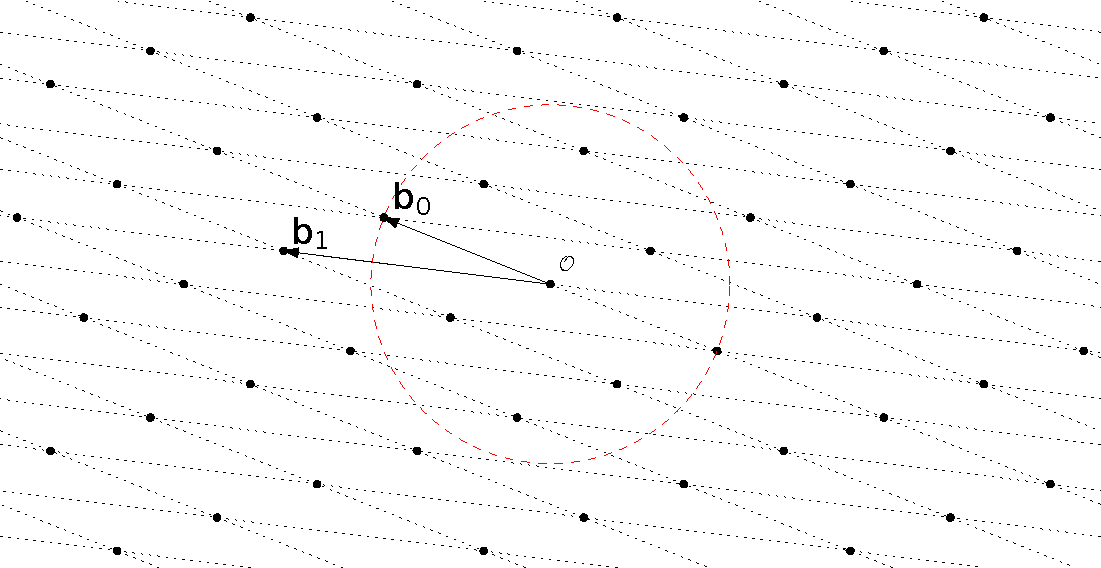
\includegraphics[width=.9\linewidth]{./assets/lattice-enumeration-0-radius.pdf}
\end{center}

\tiny Picture credit: Joop van de Pol
\end{frame}

\begin{frame}[label={sec:org1a370b2}]{Enumeration II -- Project basis}
\begin{center}
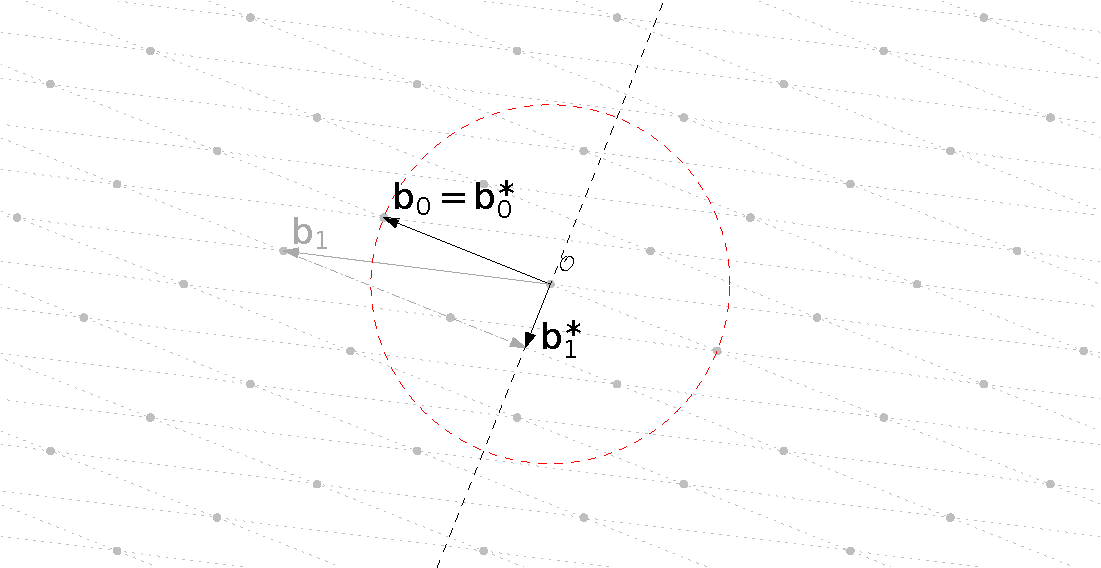
\includegraphics[width=.9\linewidth]{./assets/lattice-enumeration-1-project.pdf}
\end{center}

\tiny Picture credit: Joop van de Pol
\end{frame}

\begin{frame}[label={sec:org3a6a3e4}]{Enumeration III -- Project lattice}
\begin{center}
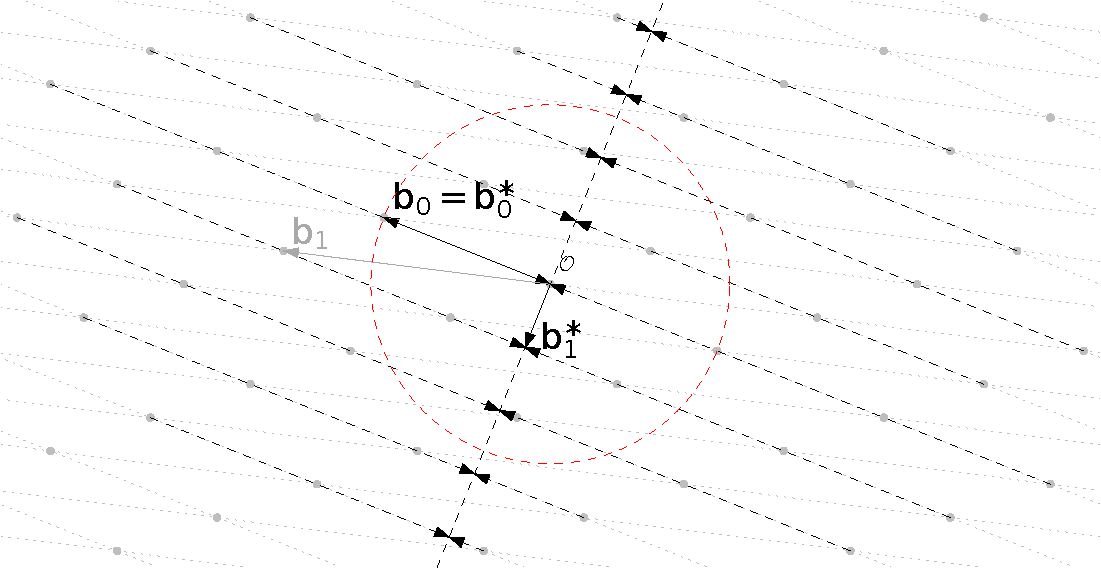
\includegraphics[width=.9\linewidth]{./assets/lattice-enumeration-2-project.pdf}
\end{center}

\tiny Picture credit: Joop van de Pol
\end{frame}

\begin{frame}[label={sec:org1602a61}]{Enumeration IV -- Enumerate projections}
\begin{center}
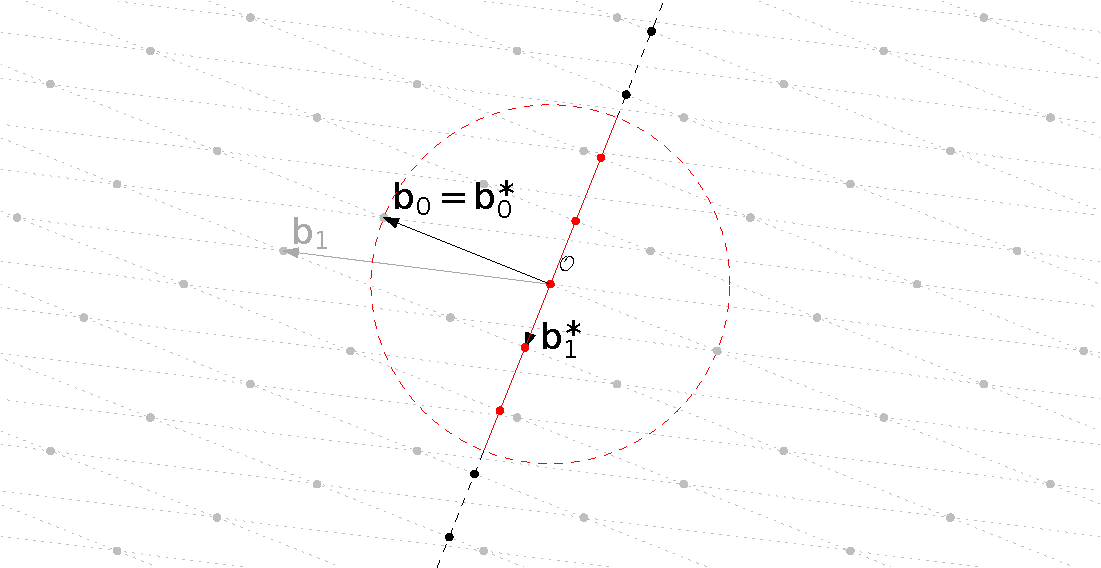
\includegraphics[width=.9\linewidth]{./assets/lattice-enumeration-3-enumerate.pdf}
\end{center}

\tiny Picture credit: Joop van de Pol
\end{frame}

\begin{frame}[label={sec:org6ea99c8}]{Enumeration V -- For each lift and enumerate}
\begin{center}
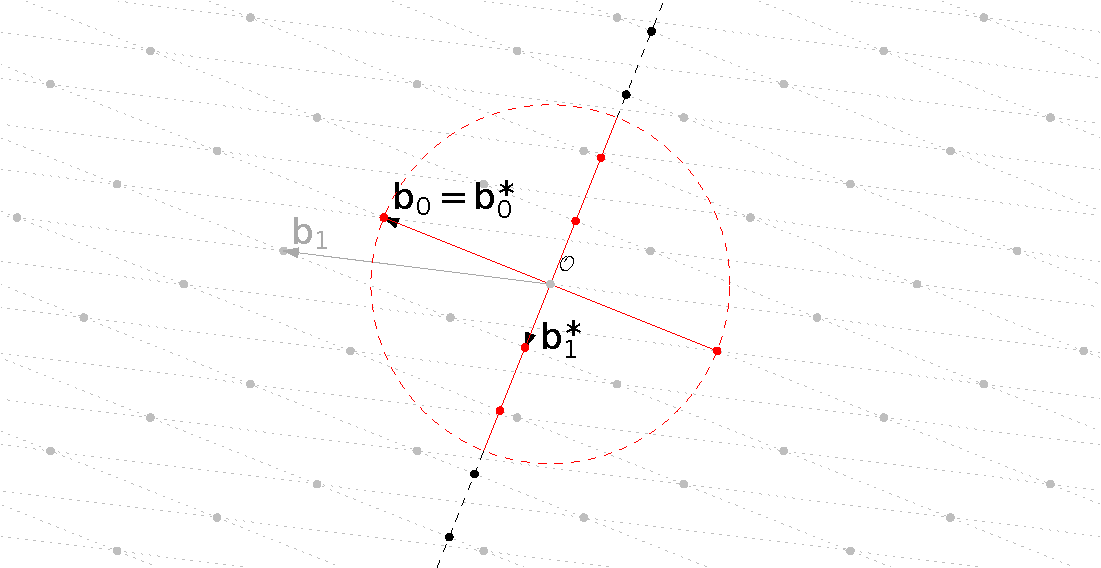
\includegraphics[width=.9\linewidth]{./assets/lattice-enumeration-4-lift.pdf}
\end{center}

\tiny Picture credit: Joop van de Pol
\end{frame}

\begin{frame}[label={sec:orgd9832ca}]{Enumeration V -- For each lift and enumerate}
\begin{center}
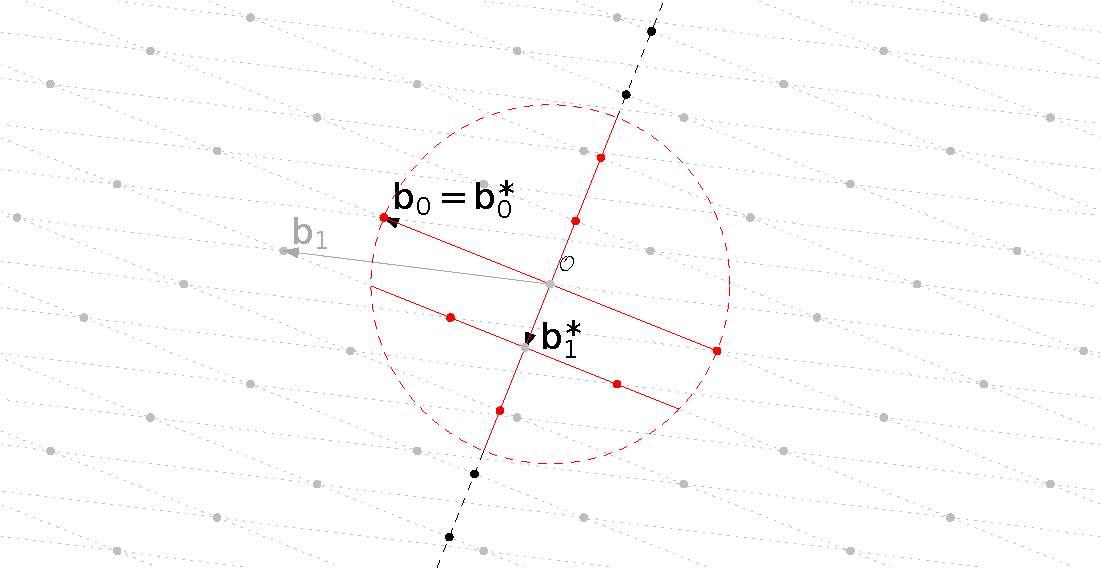
\includegraphics[width=.9\linewidth]{./assets/lattice-enumeration-5-lift.pdf}
\end{center}

\tiny Picture credit: Joop van de Pol
\end{frame}

\begin{frame}[label={sec:org0e1af8d}]{Enumeration VI -- Keep shortest}
\begin{center}
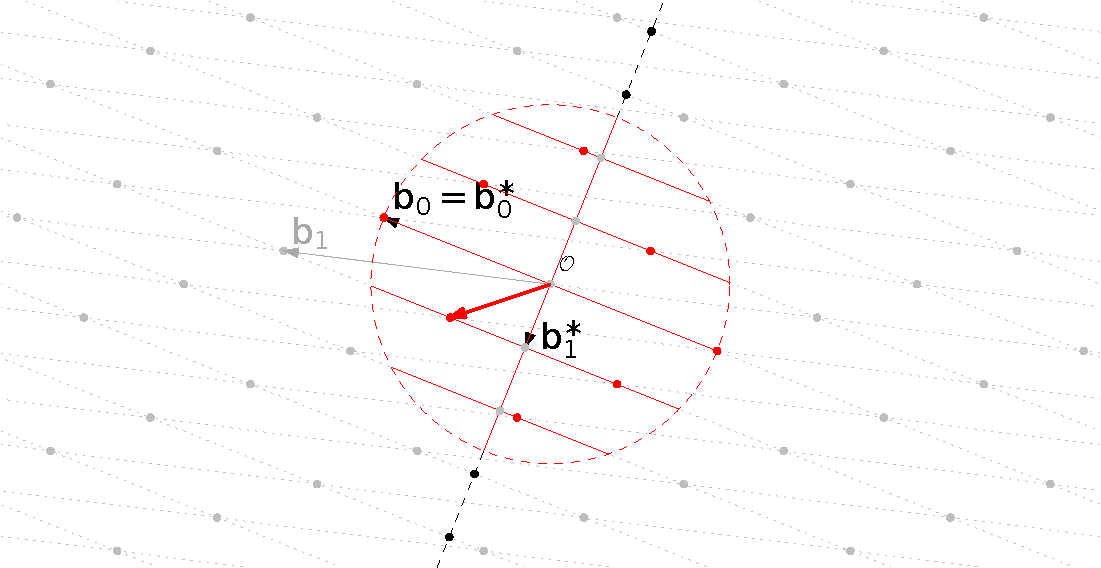
\includegraphics[width=.9\linewidth]{./assets/lattice-enumeration-6-keep.pdf}
\end{center}

\tiny Picture credit: Joop van de Pol
\end{frame}

\begin{frame}[label={sec:org25d64a3}]{Fast Enumeration}
\begin{itemize}
\item Do not exhaust the search space, but focus on a fraction with exponentially small probability of success, repeat exponentially often: speed-up \(2^{\Theta(\beta)}\)
\item Preprocess the basis with BKZ-\(\beta'\) for some \(\beta' \leq \beta\) before enumerating.
\end{itemize}
\end{frame}

\begin{frame}[label={sec:org3b0c805},fragile]{Practical Performance (Simulation)}
 \tikzset{external/export=true}
\tikzsetnextfilename{enumeration-cost-ahsvp}
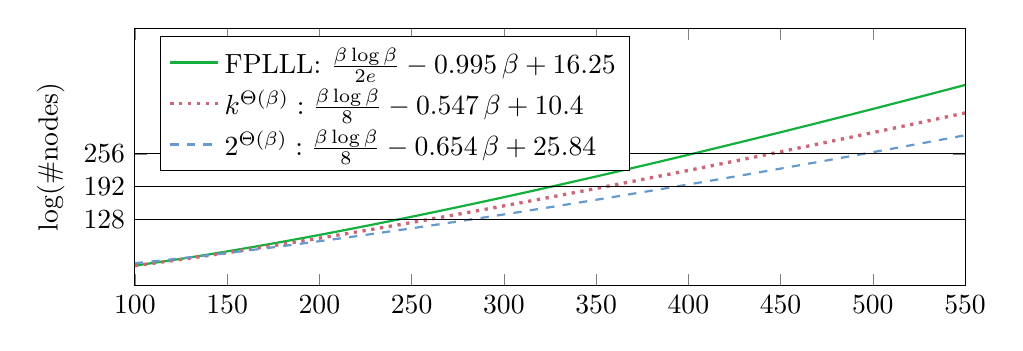
\begin{tikzpicture}
  \begin{axis}[
    legend pos = north west, 
    xmin=100, xmax=550,
    ymin=0, ymax=500,
    height=0.4\textwidth,
    ylabel = \(\log(\#\textnormal{nodes})\),
    ytick = {128,192,256},
    ]
    \addplot+ [domain=100:550, samples=250]{0.1839*x*log2(x) - 0.995*x + 16.25};
    \addlegendentry{FPLLL: \(\frac{\beta \log \beta}{2e} - 0.995\,\beta + 16.25\)};

    \addplot+ [domain=100:550, samples=250]{0.125*x*log2(x) - 0.547*x+10.4};
    \addlegendentry{\(k^{\Theta(\beta)}: \frac{\beta \log \beta}{\alert{8}} - 0.547\,\beta + 10.4\)};

    \addplot+ [domain=100:550,samples=250]{0.125*x*log2(x) - 0.654*x+25.84};
    \addlegendentry{\(2^{\Theta(\beta)}: \frac{\beta \log \beta}{8} - \alert{0.654}\,\beta + 25.84\)};

    \addplot+ [domain=100:550, samples=200, solid, thin,draw=black]{128};
    \addplot+ [domain=100:550, samples=200, solid, thin,draw=black]{192};
    \addplot+ [domain=100:550, samples=200, solid, thin,draw=black]{256};
  \end{axis}
\end{tikzpicture}
\tikzset{external/export=false}

\lstset{language=Python,label= ,caption= ,captionpos=b,numbers=none}
\begin{lstlisting}
beta, d = 500, 1000
RC.CheNgu12(beta, d).log(2), RC.ABFKSW20(beta, d).log(2), RC.ABLR21(beta, d).log(2)
\end{lstlisting}

\begin{verbatim}
(365.668328064860, 316.227302076042, 278.167302076042)
\end{verbatim}


\footnotesize \cite{AC:CheNgu11,C:ABFKSW20,C:ABLR21}
\end{frame}


\begin{frame}[label={sec:orgf5791a8}]{Sieving: Key Idea I}
\tikzset{external/export=true}
\tikzsetnextfilename{sieving-idea-1}
\centering
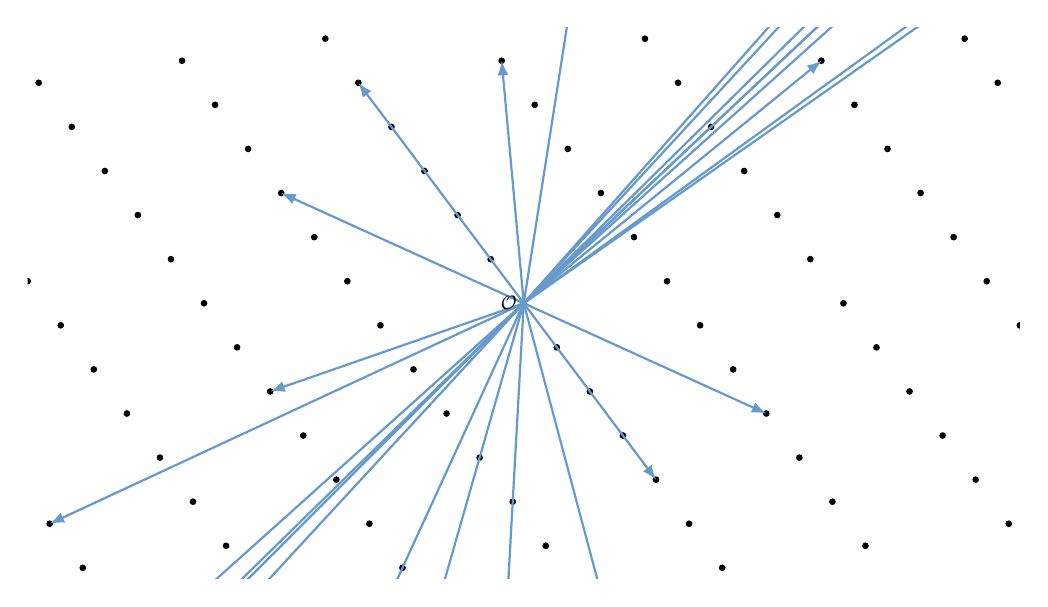
\begin{tikzpicture}[scale=0.7, every node/.style={scale=0.7}]
  \coordinate (Origin)   at (0,0);

  \clip (-9,-5) rectangle (9,5);
  \pgftransformcm{1}{0.6}{0.7}{1}{\pgfpoint{0cm}{0cm}}

  \foreach \x in {-10,-9,...,10}{%
    \foreach \y in {-10,-9,...,10}{%
      \node[draw,circle,inner sep=1pt,fill] at (2*\x,2*\y) {};
    }
  }
  % \draw [ultra thick,-latex,red] (Origin)
  % -- (Bone) node [above left] {$b_1$};
  % \draw [ultra thick,-latex,red] (Origin)
  % -- (Btwo) node [below right] {$b_2$};

  \foreach \x in {-5,-3,2,4,5}{%
    \foreach \y in {-6,-4,1,4,5}{%
      \draw [thick,-latex,DarkBlue] (Origin)
      -- (2*\x,2*\y) {};
    }
  }

  \node [left] at (Origin) {$\mathcal{O}$};
\end{tikzpicture}
\tikzset{external/export=false}
\end{frame}

\begin{frame}[label={sec:org5829ad2}]{Sieving: Key Idea II}
\tikzset{external/export=true}
\tikzsetnextfilename{sieving-idea-2}
\centering
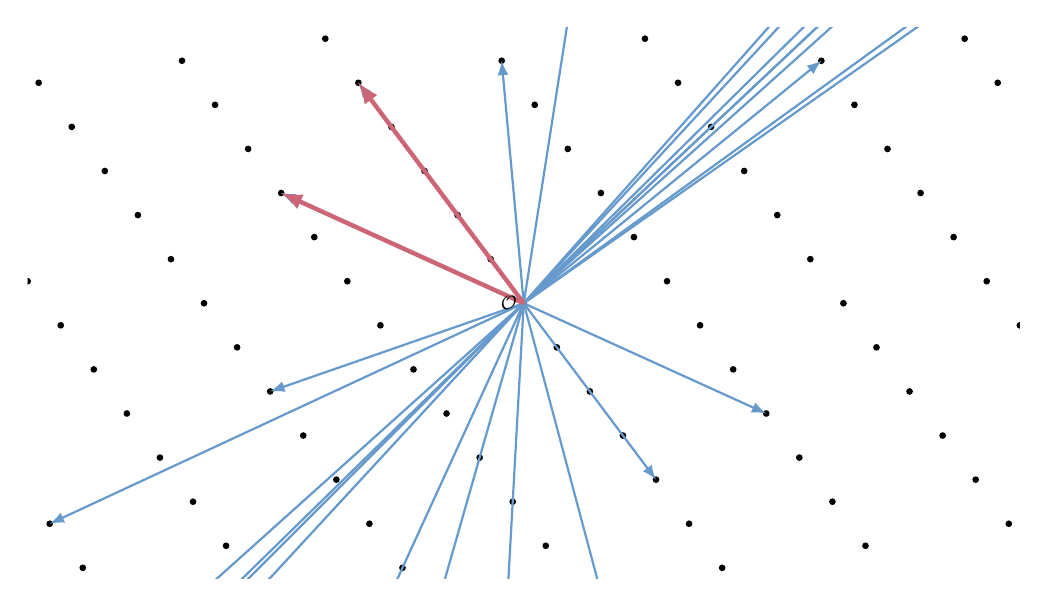
\begin{tikzpicture}[scale=0.7, every node/.style={scale=0.7}]
  \coordinate (Origin)   at (0,0);

  \clip (-9,-5) rectangle (9,5);
  \pgftransformcm{1}{0.6}{0.7}{1}{\pgfpoint{0cm}{0cm}}

  \foreach \x in {-10,-9,...,10}{%
    \foreach \y in {-10,-9,...,10}{%
      \node[draw,circle,inner sep=1pt,fill] at (2*\x,2*\y) {};
    }
  }

  \foreach \x in {-5,-3,2,4,5}{%
    \foreach \y in {-6,-4,1,4,5}{%
      \draw [thick,-latex,DarkBlue] (Origin)
      -- (2*\x,2*\y) {};
    }
  }

  \draw [ultra thick,-latex,LightRed] (Origin) -- (-10,10) {};
  \draw [ultra thick,-latex,LightRed] (Origin) -- (-10,8) {};

  \node [left] at (Origin) {$\mathcal{O}$};
\end{tikzpicture}
\tikzset{external/export=false}
\end{frame}

\begin{frame}[label={sec:orgde64d04}]{Sieving: Key Idea III}
\tikzset{external/export=true}
\tikzsetnextfilename{sieving-idea-3}
\centering
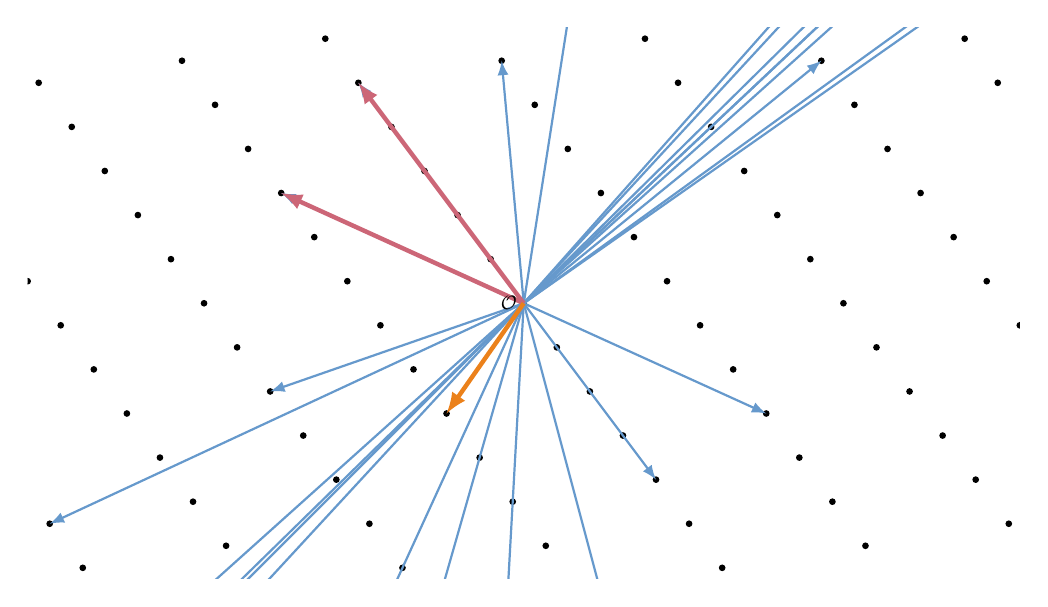
\begin{tikzpicture}[scale=0.7, every node/.style={scale=0.7}]
  \coordinate (Origin)   at (0,0);

  \clip (-9,-5) rectangle (9,5);
  \pgftransformcm{1}{0.6}{0.7}{1}{\pgfpoint{0cm}{0cm}}

  \coordinate (Bone) at (0,2);
  \coordinate (Btwo) at (2,-2);

  \foreach \x in {-10,-9,...,10}{%
    \foreach \y in {-10,-9,...,10}{%
      \node[draw,circle,inner sep=1pt,fill] at (2*\x,2*\y) {};
    }
  }

  \foreach \x in {-5,-3,2,4,5}{%
    \foreach \y in {-6,-4,1,4,5}{%
      \draw [thick,-latex,DarkBlue] (Origin)
      -- (2*\x,2*\y) {};
    }
  }

  \draw [ultra thick,-latex,LightRed] (Origin) -- (-10,10) {};
  \draw [ultra thick,-latex,LightRed] (Origin) -- (-10,8) {};
  \draw [ultra thick,-latex,LightBrown] (Origin) -- (0,-2) {};

  \node [left] at (Origin) {$\mathcal{O}$};
\end{tikzpicture}
\tikzset{external/export=false}
\end{frame}

\begin{frame}[label={sec:org1d67240}]{Sieving: Basic (Gauss) Sieve Complexity}
\begin{itemize}
\item Assume all vectors have (roughly) the same length
\item Normalise to unit sphere \(\mathcal{S}^{d-1} \coloneqq \{\vec{x} \in \RR^{d} | \|\vec{x}\| = 1\}\)
\item We have \(\|\vec{v} - \vec{w}\| \leq 1\) iff \(\left\langle \vec{v}, \vec{w} \right\rangle \ge 1/2 = \cos(\pi/3)\)
\item The probability that two random \(\vec{v}, \vec{w} \in \mathcal{S}^{d-1}\) satisfy \(\left\langle \vec{v}, \vec{w} \right\rangle \ge 1/2\) is
\[= \poly[d] \cdot {\left(\frac{4}{3}\right)}^{d/2} \approx 2^{0.2075\,d + o(d)}\]
\item Need \(\poly[d] \cdot {\left(\frac{4}{3}\right)}^{d/2}\) vectors, comparing all pairs costs \(\poly[d] \cdot {\left(\frac{4}{3}\right)}^{d} \approx 2^{0.4150\,d + o(d)}\).
\end{itemize}


\footnotesize \fullcite{SODA:MicVou10}
\end{frame}

\begin{frame}[label={sec:orgf3e9552}]{Sieving: Buckets I}
\tikzset{external/export=true}
\tikzsetnextfilename{sieving-buckets}
\centering
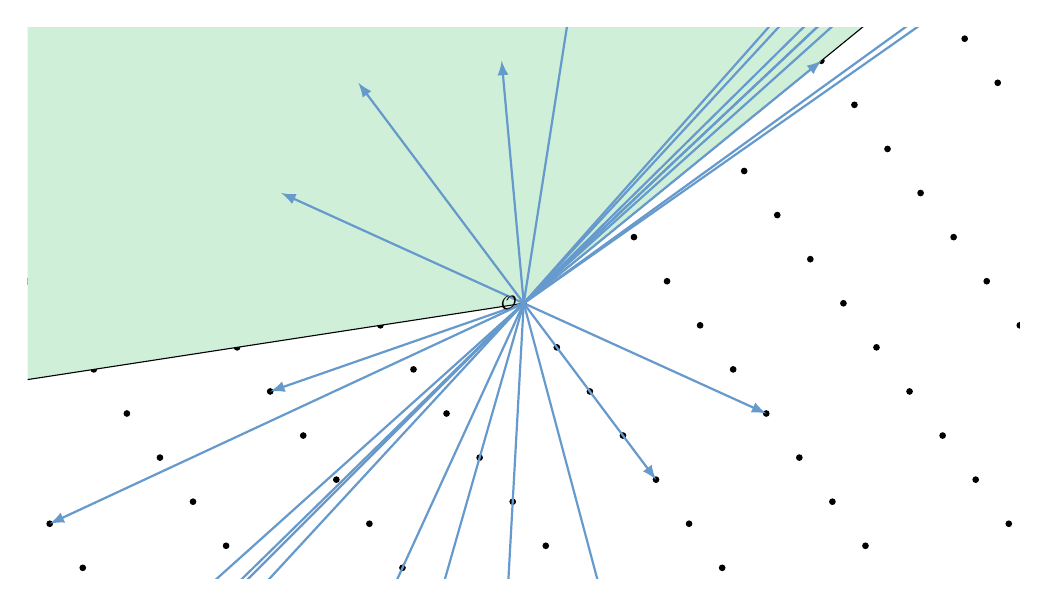
\begin{tikzpicture}[scale=0.7, every node/.style={scale=0.7}]
  \coordinate (Origin)   at (0,0);

  \clip (-9,-5) rectangle (9,5);
  \pgftransformcm{1}{0.6}{0.7}{1}{\pgfpoint{0cm}{0cm}}

  \coordinate (Bone) at (0,2);
  \coordinate (Btwo) at (2,-2);

  \foreach \x in {-10,-9,...,10}{%
    \foreach \y in {-10,-9,...,10}{%
      \node[draw,circle,inner sep=1pt,fill] at (2*\x,2*\y) {};
    }
  }

\draw[fill=LightGreen!20!white] (-20,10) -- (0,0) -- (20,10) -- (-100,100) {};

\foreach \x in {-5,-3,2,4,5}{%
    \foreach \y in {-6,-4, 1,4,5}{%
      \draw [thick,-latex,DarkBlue] (Origin)
      -- (2*\x,2*\y) {};
    }
 }

  \node [left] at (Origin) {$\mathcal{O}$};
\end{tikzpicture}
\tikzset{external/export=false}
\end{frame}

\begin{frame}[label={sec:org3c8fe6e}]{Sieving: Buckets II}
If \(\vec{v}\), \(\vec{c}\) are somewhat close and \(\vec{w}\), \(\vec{c}\) are somewhat close then perhaps \(\vec{w}\), \(\vec{v}\) are close?

\begin{block}{Strategy}
\begin{itemize}
\item Sort vectors into somewhat loose buckets,
\item Do quadratic pairwise comparison only within each bucket.
\end{itemize}
\end{block}

\begin{description}
\item[{BGJ}] Split search space into buckets. \textbf{Cost}: \(2^{0.311\,\beta + o(\beta)}\).\footfullcite{EPRINT:BecGamJou15}
\item[{BDGL}] Use codes to decide which bucket to consider. \textbf{Cost}: \(2^{0.292\,\beta + o(\beta)}\). \footfullcite{SODA:BDGL16}
\end{description}
\end{frame}

\begin{frame}[label={sec:orgd30a0d5}]{Sieving: G6K}
G6K \footfullcite{EC:ADHKPS19} is a Python/C++ framework for experimenting with sieving algorithms (inside and outside BKZ)
\begin{itemize}
\item Does not take the “oracle” view but considers sieves as stateful machines.
\item Implements several sieve algorithms
\begin{itemize}
\item Gauss and NV
\item Triple Sieve
\item BGJ1 (BGJ with one level of filtration)
\item BDGL (with one and two block respectively)
\end{itemize}
\item Applies recent tricks and adds new tricks for improving performance of sieving
\end{itemize}
\end{frame}

\begin{frame}[label={sec:org6ddd341}]{Sieving: SVP}
\begin{center}
\begin{tikzpicture}
    \begin{semilogyaxis}[ylabel=seconds, xlabel=\(\beta\), legend style={fill=}, legend pos=north west, height=0.5\textwidth]
        \addplot+ [only marks] table [x=d, y=FPLLL, col sep=comma]{data/exact-svp.csv};
        \addlegendentry{BKZ + pruned enum (FPLLL)};
        \addplot+ [only marks] table [x=d, y=G6K, col sep=comma]{data/exact-svp.csv};
        \addlegendentry{G6K WorkOut};
    \end{semilogyaxis}
\end{tikzpicture}
Average time in seconds for solving exact SVP
\end{center}
\end{frame}

\begin{frame}[label={sec:org936d072}]{Darmstadt HSVP\textsubscript{1.05} Challenges}
\begin{center}
\begin{tikzpicture}
  \begin{axis}[xlabel=\(d\),ylabel=\(\log_2(\textnormal{cycles})\),height=0.5\textwidth]
    \addplot table [x=d, col sep=comma, y expr = log2(100*\thisrowno{2}),, select coords between index={0}{50} ]{data/fplll-simulations,svp-challenge.csv};
    \addlegendentry{HSVP\(_{1.05}\) non-parallel enum sim};

    \addplot table [x=d, col sep=comma, y expr = log2(100*\thisrowno{2}), select coords between index={70}{166}]{data/fplll-simulations-enumeration-cost-2e.csv};
    \addlegendentry{SVP non-parallel enum sim};

    \addplot+ [only marks] table [unbounded coords=discard,x=d, col sep=comma, y expr = %
    log2(\thisrowno{3}*3600*2*10.0^9)%
    ]{data/svp-challenge-observations.csv};
    \addlegendentry{HoF:FK15};

    \addplot+ [only marks] table [unbounded coords=discard,x=d, col sep=comma, y expr = %
    log2(\thisrowno{4}*3600*2*10.0^9)%
    ]{data/svp-challenge-observations.csv};
    \addlegendentry{HoF:KT17};

    \addplot+ [only marks] table [unbounded coords=discard,x=d, col sep=comma, y expr = %
    log2(\thisrowno{5}*3600*2*10.0^9)%
    ]{data/svp-challenge-observations.csv};
    \addlegendentry{G6K};

  \end{axis}
\end{tikzpicture}
\end{center}
\end{frame}

\begin{frame}[label={sec:org03717da}]{GPU Sieving}
\begin{itemize}
\item Stream database of vectors to GPU
\item Run low precision inner products there
\end{itemize}

\begin{center}
\begin{tabular}{rrrrrrrrr}
\toprule
dim & TD4F & D4F & MSD & Norm & Norm/GH & FLOP & Walltime & Mem GiB\\
\midrule
158 & 31 & 29 & 129 & 3303 & 1.04329 & 262.1 & 9h 16m & 89\\
162 & 31 & 31 & 131 & 3341 & 1.04220 & 263.2 & 18h 32m & 156\\
176 & 34 & 33 & 143 & 3487 & 1.04412 & 267.5 & 12d 11h & 806\\
178 & 34 & 32 & 146 & 3447 & 1.02725 & 268.6 & 22d 18h & 1060\\
180 & 34 & 30 & 150 & 3509 & 1.04003 & 269.9 & 51d 14h & 1443\\
\bottomrule
\end{tabular}

\end{center}

\scriptsize

\fullcite{EC:DucSteWoe21}
\end{frame}

\begin{frame}[label={sec:orgcc336e2},fragile]{Try it at Home}
 \lstset{language=sage,label= ,caption= ,captionpos=b,numbers=none}
\begin{lstlisting}
from fpylll import IntegerMatrix, GSO, LLL
from fpylll.tools.bkz_stats import dummy_tracer
from g6k import Siever
from g6k.algorithms.bkz import pump_n_jump_bkz_tour

A = LLL.reduction(IntegerMatrix.random(180, "qary", k=90, bits=20))
g6k = Siever(A)

for b in range(20, 60+1, 10):
    pump_n_jump_bkz_tour(g6k, dummy_tracer, b, pump_params={"down_sieve": True})
\end{lstlisting}

\begin{description}
\item[{\url{https://github.com/fplll/g6k}}] C++ kernel + Python frontend
\item[{\url{https://github.com/WvanWoerden/G6K-GPU-Tensor}}] G6K fork adding GPU support
\end{description}
\end{frame}

\begin{frame}[label={sec:org02f27bd},fragile]{Costing Sieves}
 \begin{columns}[t]
\begin{column}{0.5\columnwidth}
"\emph{The main difference is the cost of the random product code decoding algorithm.}"

\ \\
\scriptsize

\fullcite{Matzov22}
\end{column}

\begin{column}{0.5\columnwidth}
"\emph{Concretely, we conclude on an overhead factor of about  on the number of gates in the RAM model compared to the idealized model for dimensions around  after an appropriate re-parametrization.}"

\ \\
\scriptsize

\fullcite{EPRINT:Ducas22}
\end{column}
\end{columns}

"Core-SVP" \cite{USENIX:ADPS16}: \(2^{0.292\,\beta \pm 0}\) v \cite{NISTPQC-R3:CRYSTALS-KYBER20,AC:AGPS20} v \cite{Matzov22}

\lstset{language=Python,label= ,caption= ,captionpos=b,numbers=none}
\begin{lstlisting}
RC.ADPS16(500, 1000).log(2), RC.Kyber(500, 1000).log(2), RC.MATZOV(500, 1000).log(2)
\end{lstlisting}

\begin{verbatim}
(146.000000000000, 176.547704482770, 169.704298365530)
\end{verbatim}
\end{frame}

\section{Quantum Stuff}
\label{sec:org4f10863}
\begin{frame}[label={sec:org92f6e1c}]{Quantum Estimates}
\begin{description}
\item[{{\color{LightRed} \textbf{Sieving} }}] Given some vector \(\vec{w}\) and a list of vectors \(L\), apply Grover’s algorithm to find \(\{\vec{v} \in L \textnormal{ s.t. } \|\vec{v} \pm \vec{w}\| \leq \|\vec{w}\|\}\).\footfullcite{PhD:Laarhoven15}

\item[{{\color{DarkBlue} \textbf{Enumeration} }}] Apply Montanaro’s quantum backtracking algorithm for quadratic speed-up.\footfullcite{EPRINT:AonNguShe18}
\end{description}
\end{frame}

\begin{frame}[label={sec:org99aaf76}]{Quantum Sieving}
\begin{itemize}
\item A quantum sieve needs list of \(2^{0.2075 \beta}\) vectors before pairwise search with Grover

\item Fast sieves use that the search is structured, Grover does unstructured search
\begin{itemize}
\item Quantum Gauss Sieve \[2^{(0.2075 + \frac{1}{2} 0.2075)\, \beta + o(\beta)} = 2^{0.311\, \beta + o(\beta)} \textnormal{ time},\qquad 2^{0.2075\, \beta + o(\beta)} \textnormal{ memory}\]
\item Classical BGJ Sieve \footfullcite{EPRINT:BecGamJou15} \[\phantom{2^{(0.2075 + \frac{1}{2} 0.2075)\, \beta + o(\beta)} = }2^{0.311\, \beta + o(\beta)}\textnormal{ time}, \qquad 2^{0.2075\, \beta + o(\beta)} \textnormal{ memory}\]
\end{itemize}
\item Asymptotically fastest sieves have small lists and thus less Grover speed-up potential
\end{itemize}
\end{frame}

\begin{frame}[label={sec:org2b6bedf}]{Implementing Quantum Algorithms for SVP: Sieving (Underestimates)}
\tikzset{external/export=true}
\tikzsetnextfilename{quantum-sieving-bdgl-ge}
\tikzpicturedependsonfile{data/cost-estimate-list_decoding-classical.csv}
\tikzpicturedependsonfile{data/cost-estimate-list_decoding-ge19.csv}
\begin{tikzpicture}
  \begin{axis}[ylabel={$\log_{2}(\#ops)$}, height=0.5\textwidth,xlabel=,]
    \addplot+[] table [x=d, col sep=comma, y=log_cost] {data/cost-estimate-list_decoding-classical.csv};
    \addlegendentry{BDGL (c: RAM)};

    \addplot+[] [domain=64:1024] {0.2924*x};
    \addlegendentry{\(0.2924\,d\)};

    \addplot+[] table [x=d, col sep=comma, y=log_cost] {data/cost-estimate-list_decoding-ge19.csv};
    \addlegendentry{BDGL (q: Gidney and Ekerå 2019)};

    \addplot+[] [domain=64:1024] {0.2652*x};
    \addlegendentry{\(0.2652\,d\)};
  \end{axis}
\end{tikzpicture}
\tikzset{external/export=false}


\scriptsize{

\fullcite{AC:AGPS20}

}
\end{frame}

\begin{frame}[label={sec:org5e11d37}]{Quantum estimates do not seem to matter}
\begin{itemize}
\item The resistance of post-quantum algorithms to quantum computers is routinely, e.g. in the NIST PQC Standardization Process, compared to that of the AES family of block ciphers.
\item The state of the art is that AES-\(\lambda\) resists classical attacks of cost \(\approx 2^{\lambda}\) and quantum attacks of cost \(\approx 2^{\lambda/2}\), the latter being due to Grover's algorithm.\footnote{See \cite{EC:JNRV20} for more detailed cost estimates}
\item Parameters for post-quantum schemes are chosen such that they resist known classical attacks of cost \(\approx 2^{\lambda}\) and known quantum attacks of cost \(\approx 2^{\lambda/2}\) and any algorithm with complexity \(\gg 2^{\lambda/2}\) will not affect the claimed security level.
\end{itemize}
\end{frame}


\begin{frame}[label={sec:org5453dbc}]{Other Approaches}
\begin{description}
\item[{BKW}] combinatorial technique, relatively efficient for small secrets
\item[{Arora-Ge}] use Gröbner bases, asymptotically efficient , but large constants in the exponent
\end{description}

\begin{alertblock}{Rule of Thumb}
Don’t need to worry about these unless secret is unusually small (e.g. ternary) and/or sparse.
\end{alertblock}
\end{frame}

\begin{frame}[label={sec:org2288f43},standout]{Fin \& Obligatory "We're hiring" Slide}
\begin{center}
\Huge \alert{Thank You}
\end{center}

From 2023 I will work for\\
King's College London and for SandboxAQ.

\begin{description}
\item[{KCL}] will recruit academic staff, (maybe postdocs) and PhD students (not limited to post-quantum)
\item[{SandboxAQ}] will recruit staff, postdocs, PhD students and interns
\end{description}
\end{frame}

\begin{frame}[allowframebreaks]{References}
\renewcommand*{\bibfont}{\scriptsize}
\printbibliography[heading=none]
\end{frame}
\end{document}